\chapter{Комплексы программ} \label{chap:exm}
\section{Библиотека тензорных вычислений t3f} \label{sec:t3f}
Для выполнения численных расчетов с использованием разложения в Тензорный Поезд, автором был разработан программный пакет на языке Python. Главные отличия от уже существующих реализаций разложения в Тензорный Поезд[CITE] составляют:
\begin{enumerate}
	\item Поддержка работы на графических ускорителях (GPU) для всех операций. Пакет автоматически проверяет доступно ли на данной машине устройство GPU и если доступно, переносит расчеты на графический ускоритель.
	\item Расширенная поддержка Римановой оптимизации. Единственный альтернативный пакет в котором есть поддержка Римановой оптимизации это TTPY, в котором есть только операция проекции на касательное пространство (которая была реализована в этом пакете автором данной диссертации). В пакете T3F доступно множество частных случаев требующихся для реализации численных методов Римановой оптимизации, которые формально могут быть реализованы с помощью комбинации оператора проекции и базовых операций таких как матрично-векторное умножение, но при реализации этих частных случаев в отдельной функции позволяют значительно ускорить вычисления. Примерами таких операций являются проекция матрично-вектороного произведения на касательную плоскость ТТ-вектора $P_b(A c)$ и вычисления матрицы Грама проекций на касательную плоскость $G_{ij} = <P_b(x_i), P_b(x_j)>$.
	\item Поддержка работа с множеством (батчем) ТТ-объектов одновременно, реализованная с помощью векторизованных операций. Например подсчет матрицы Грама набора ТТ-объектов можно выполнить одной параллельной операцией.
	\item Поддержка автоматического дифференцирования произвольной функции ошибки $L(\cdot)$ являющейся функцией от тензора в ТТ-формате.
	\item Документация и тесты (покрытие тестами составляет 93\% при общем объеме кода в 10000 строк).
\end{enumerate}

\subsection{Интерфейс программного кода}
В листинге~\ref{list:t3f-example} приведен пример простой программы, которая выполняет факторизацию двух данных тензоров в формат тензорного поезда, складывает полученные ТТ-объекты, и округляет результат.
\begin{ListingEnv}[!h]% настройки floating аналогичны окружению figure
%    \captionsetup{format=tablenocaption}% должен стоять до самого caption
    \caption{Представление тензоров в формат Тензорного Поезда а так же другие операции с помощью библиотеки T3F.}
    % далее метка для ссылки:
    \label{list:t3f-example}
    % окружение учитывает пробелы и табуляции и применяет их в сответсвии с настройками
    \begin{lstlisting}[language={Python}]
# Import the main package.
import t3f
# Import a supplementary tool.
import numpy as np

# Generate random tensors of size 3 x 4 x 5.
tens_1 = np.random.randn(3, 4, 5)
tens_2 = np.random.randn(3, 4, 5)

# Convert the tensors into the TT-format with TT-ranks 10 and 20.
tt_1 = t3f.to_tt_tensor(tens_1, max_r=10)
tt_2 = t3f.to_tt_tensor(tens_2, max_r=20)

# Sum the TT-objects and round the result to have TT-rank 5.
tt_res = t3f.round(tt_1 + tt_2, max_r=5)

# Convert the result into a full (uncompressed) tensor.
res = t3f.full(tt_res)
    \end{lstlisting}
\end{ListingEnv}%

\subsection{Список поддерживаемых операций}
Список некоторых поддерживаемых операций и их описание доступно в таблице~\ref{tbl:t3f-ops}.

%\fontsize{10pt}{10pt}\selectfont
\begin{longtable}[c]{ll} %longtable* появляется из пакета caption и даёт ненумерованную таблицу
 \caption{Список некоторых операций поддерживаемых библиотекой T3F. Полный список доступ по адресу \url{https://t3f.readthedocs.io/en/latest/}.}\label{tbl:t3f-ops}\\
%\\ 
 \hline
 %\multicolumn{4}{|c|}{\textbf{Файл puma\_namelist}}        \\ \hline
 Функция & Описание               \\ \hline
                                              \endfirsthead   \hline
 \multicolumn{2}{|c|}{\small\slshape (продолжение)}        \\ \hline
 Функция & Описание               \\ \hline
                                              \endhead        \hline
% \multicolumn{4}{|c|}{\small\slshape (окончание)}        \\ \hline
% Параметр & Умолч. & Тип & Описание               \\ \hline
%                                             \endlasthead        \hline
 \multicolumn{2}{|r|}{\small\slshape продолжение следует}  \\ \hline
                                              \endfoot        \hline
                                              \endlastfoot
to\_tt\_tensor(a) & Факторизует тензор а в формат Тензорного Поезда.\\
to\_tt\_matrix(a) & Факторизует матрицу а в матричный ТТ-формат.\\
round(a, rank) & Возвращает ТТ-представление переданного ТТ-объекта\\
&  округленного до TT-ранга rank.\\
add(a, b) & Возвращает ТТ-представление одного тензора или матрицы\\
&  или батча тензоров или матриц поэлементной суммы a и b.\\
multiply(a, b) & Возвращает ТТ-представление одного тензора или матрицы \\
 & или батча тензоров или матриц поэлементного произведения \\
 & аргументов a и b.\\
add\_n\_projected(a, b) & Возвращает ТТ-представление поэлементной суммы\\
 & аргументов. Работает только для элементов одного\\
 & касательного пространства, но в отличие от t3f.add\\
 & не увеличивает ТТ-ранг.\\
flat\_inner(a, b) & Скалярное произведение двух ТТ-матриц или ТТ-тензоров. \\
& В случае если один из аргументов -- это батч объектов, \\
& возвращает вектор скалярных произведений.\\
frobenius\_norm(a, & Норма Фробениуса аргумента. В случае переданный \\
~~~epsilon, & аргумент это батч объектов, возвращает вектор \\\\
~~~differentiable) & Фробениусовых норм. Добавляет переданный epsilon под корень для численной стабильности. Поддерживает два режима вычисления -- через QR разложение (differentiable=False) и через произведения ядер.\\
full(a) & Превращает переданный ТТ-объект в полный формат.\\
gather\_nd(a, & Параллельный доступ к элементов ТТ-объекта а по \\
~~~indices) &  индексам indices. То-есть \\
& out[i] = a[indices[i, 0], indices[i, 1], …].\\
gram\_matrix(a) & Матрица Грама переданного батча ТТ-объектов,\\
& вычисляется параллельно.\\
matmul(a, b) & Матричное умножение двух объектов. Поддерживается\\
&  умножение между двумя ТТ-матрицами, \\
& ТТ-матрицей и обычной матрицей и ТТ-матрицей и разреженной матрицей. Если один из аргументов -- это батч объектов, результатом будет батч матричных умножений выполненных параллельно.\\
pairwise\_flat\_inner( & Вычисление матрицы скалярных произведений между \\
~~~a, b, matrix=None) & батчами ТТ-объектов a и b. Если передан аргумент matrix, \\
& то вычисляется скалярное произведение заданное переданной матрицей, out[i, j] = $\langle a[i], matrix b[j] \rangle$.\\
%pairwise\_flat\_inner\_projected(a, b) & Вычисление матрицы скалярных произведений между батчами ТТ-объектов a и b в предположении что все объекты лежат в одном касательном пространстве. Работает быстрее общего метода pairwise\_flat\_inner.\\
project(what, where) & Вычисляет проекцию ТТ-объекта what на касательное \\
& пространство в точке ТТ-объекта where. В случае, если what представляет собой батч ТТ-объектов, результатом будет батч проекций каждого из элементов в батче what вычисленных параллельно.\\
project\_matmul( & Вычисляет проекцию матричного произведения matrix what \\
~~~what, where & на касательное пространство в точке ТТ-объекта where. \\
, matrix) & В случае, если what представляет собой батч ТТ-объектов, \\
& результатом будет батч проекций каждого из элементов в батче matrix what вычисленных параллельно. Работает быстрее чем последовательность из матричного умножения и проекции project(matmul(matrix, what), where).\\
project\_sum(what, & Вычисляет сумму проекций ТТ-объектов в батче what на касательное пространство\\
~~~where, weights) & в точке ТТ-объекта where. В случае если передан параметр weights, вычисляет взвешанную сумму. Работает параллельно по числу объектов.\\
\alert{quadratic\_form}( & Вычисляет билинейную форму $out[i] = \langle a[i], A b[i] \rangle$\\
~~~ A, b, c) & параллельно по числу ТТ-объектов в батчах b и c.\\
transpose(A) & Возвращает ТТ-представление матрицы транспонированния \\
& матрицы А.\\
% \hline 
\end{longtable}
%\normalsize% возвращаем шрифт к нормальному







\subsection{Быстродействие пакета}
Для оценки быстродействия пакета T3F, была сгенерирована случайная матрица в ТТ формате размера $10^{10} \times 10^{10}$ с 10 ядрами и ТТ-рангами равными $10$, a так же случайный ТТ-векторов (матриц размера $10^{10} \times 1$) так же с ТТ рангами равными 10. Было замерено время работы матрично-векторного умножения (`матвек`), матрично-матричного умножения (`матмул`), вычисления нормы Фробениуса (`норма`) и вычисление матрицы Грама (`Грам`). Каждая операция была выполнена для одного объекта (например умножение одной матрицы на один вектор) и для батча из 100 объектов (например умножение одной матрицы на 100 различных векторов). В случае матрицы Грама, применение операции к одному объекту означает вычисление скалярного произведения вектора на себя, а в случае батча из 100 объектов вычисление матрицы Грама размера $100 \times 100$. Две последнии операции были проведены на тензорах ТТ ранга 100: округление тензора размера $10^{10}$ c TT-ранга 100 до ТТ-ранга 10 и проекция тензора ТТ-ранга 100 на касательную плоскость тензора ТТ-ранга 10 (см. Тбл.~\ref{tbl:t3f-benchmark}).
\begin{center}
\begin{table}%[!htbp]
  \begin{tabular}{  l c c  c  c c}
    \hline
%     Op & TTPY & 1 object CPU & 1 object GPU & 100 objects CPU & 100 objects GPU  \\ \hline
    \multirow{3}{1.8cm}{\centering  Op } & \multirow{3}{2.2cm}{\centering TTPY \\ 1 объект \\ CPU} & \multirow{3}{2.2cm}{\centering T3F \\ 1 объект \\ CPU } & \multirow{3}{2.2cm}{\centering T3F \\ 1 объект \\ GPU } & \multirow{3}{2.9cm}{\centering T3F \\ 100 объектов \\ CPU } & \multirow{3}{2.9cm}{\centering T3F \\ 100 объектов \\ GPU }  \\[1.5cm] \hline
    матвек          &            11.142 &       0.129 &       0.121 &         0.003 &         0.003 \\
матмул          &            86.191 &       0.125 &       0.133 &         0.004 &         0.004 \\
нормы            &             3.790 &       1.902 &       0.893 &         0.422 &         0.050 \\
Грам            &             0.145 &       0.806 &       0.703 &         0.029 &         0.001 \\
округление           &            73.027 &       0.159 &       0.165 &         0.006 &         0.006 \\
проекция &           116.868 &       1.564 &       1.658 &         0.017 &         0.018 \\
    \hline
  \end{tabular}
  \caption{Время работы в мс различных операций в библиотеке TTPY и в библиотеке T3F на CPU и на GPU. Время работы для батча из 100 объектов приведено в расчете на один объект, т.е. например выполнение 100 матрично-векторных умножений (`матвек`) на CPU занимает 0.3 мс, но в таблице приведено время 0.003 в пересчете на один объект. Замеры времени проводились на сервере NVIDIA DGX-1 с графическими ускорителями Tesla V100 GPU (при расчете использовался только один графический ускоритель) и процессором Intel(R) Xeon(R) CPU E5-2698 v4 @ 2.20GHz с 80 логическими ядрами в двойной точности. \label{tbl:t3f-benchmark}}
\end{table}
\end{center}

\subsection{Реализация новых операций и их асимптотическая сложность}
В этом разделе описаны детали реализации операций, которые были впервые разработаны в рамках пакета T3F а так же проведен анализ асимптотической сложности их работы. Операции приведенные ниже используются в методе поиска собственных значений эрмитовых матриц~(раздел~\ref{sec:quantum-solver}) и в работе~\cite{izmailov2018scalable}.


\paragraph{Проекция матрично-векторного умножения}
Проекцию матрично-векторного умножения на касательное пространство ТТ-вектора $P_{T_{\vec{w}} \mathcal{M}_{\rank}} (\mat{A}\vec{b})$ для батча ТТ-векторов $\vec{b}$ длины $b$ можно реализовать использую последовательность из двух операций: матрично-векторное умножение и проекцию за асимптотическую сложность $\compl(b d \rank_{\mat{A}} \rank_{\vec{b}} n (r_A \rank_{\vec{b}} (\rank_{\vec{w}} + n) + \rank_{\vec{w}}^2))$. Однако, в часто встречающемся на практике случае когда $\rank_{\vec{w}} < \rank_{\vec{b}}$, эти две операции можно объединенить в одну чтобы выполнить их асимптотически быстрее за $\compl(b d \rank_{\mat{A}} \rank_{\vec{w}} n (r_A \rank_{\vec{w}} (\rank_{\vec{b}} + n) + \rank_{\vec{b}}^2)$ операций. В библиотеке T3F быстрая версия данной операции доступна в виде функции \texttt{t3f.project\_matmul(b, w, A)}.

Для реализации быстрой версии проекции матрично-векторного умножения, рассмотрим определение операции проекции (см. раздел~\ref{sec:riemannian-help})
\begin{equation}
\label{eq:projection-def}
\delta \widetilde{\mat{U}}_k^L = (I_{\rank_{k-1}n_k} - \mat{U}^L_k (\mat{U}^L_k)^\intercal) (I_{n_k} \otimes \mat{W}_{\leq k-1})^\intercal \mat{Z}^{\langle k \rangle} \mat{W}_{\geq k+1}	
\end{equation}
Пусть тензор $\tens{Z}$ представлен в ТТ-формате. Тогда~\eqref{eq:projection-def} можно переписать следующим образом
%\begin{equation*}
%\delta \widetilde{\mat{U}}_k[j](\gamma_1, \gamma_2) = (\delta(\alpha_{k-1} - \beta_1)\delta(i_k - j) - \sum_{\beta_3} U_k[j](\beta_1, \gamma_3) \mat{U}_k[i_k](\alpha_{k-1}, \gamma_3) (\delta(i_k - j) U_1[i_1](\alpha_{0}, \alpha_1) \ldots U_{k-1}[i_{k-1}](\alpha_{k-1}, \alpha_k) G_1^{\tens{Z}}[i_1](\beta_0, \beta_1)\ldots G_{d}^{\tens{Z}}[i_d](\beta_{d-1}, \beta_d) U_{k+1}[i_{k+1}](\alpha_{k}, \alpha_{k+1}) \ldots U_{d}[i_{d}](\alpha_{d-1}, \alpha_d)
%\end{equation*}
\begin{equation*}
\begin{aligned}
\delta \widetilde{\mat{U}}_k[j] = \sum_{i_1, \ldots, i_d}(I_{\rank_{k-1}}\delta(j - i_k) - \mat{U}_k[j] (\mat{U}_k[i_k])^\intercal) \overbrace{(\mat{U}_1[i_1] \ldots \mat{U}_{k-1}[i_{k-1}])^\intercal}^{\vec{a} \text{ размера } r_{k-1}(\tens{W}) \times 1} \cdot\\
\cdot \underbrace{\mat{G}_1^{\tens{Z}}[i_1]\ldots \mat{G}_{k-1}^{\tens{Z}}[i_{k-1}]}_{\vec{e}^\intercal \text{ размера } 1 \times \rank_{k-1}(\tens{Z})} \mat{G}_{k}^{\tens{Z}}[i_k] \underbrace{\mat{G}_{k+1}^{\tens{Z}}[i_{k+1}]\ldots \mat{G}_{d}^{\tens{Z})}[i_d]}_{\vec{f} \text{ размера } \rank_{k}(\tens{Z}) \times 1} \cdot \underbrace{(\mat{V}_{k+1}[i_{k+1}] \ldots \mat{V}_{d}[i_{d}])^\intercal}_{\vec{g}^\intercal \text{ размера } 1 \times r_k(\tens{W})}
\end{aligned}
\end{equation*}
Рассмотрим внешнее произведение векторов $\vec{a} \vec{e}^\intercal$ (которые вообще говоря зависят от индексов $\vec{a} = \vec{a}_{k-1}[i_1, \ldots, i_{k-1}]$, но эта зависимость была опущена для упрощения обозначений). Вытянув матрицу результата произведения в вектор, можно переписать результат через кронекрово произведение $\text{vec}(\vec{a} \vec{e}^\intercal)^\intercal = \vec{a}^\intercal \otimes \vec{e}^\intercal$, и наоборот, результат внешнего произведения можно получить преобразовав кронекерово произведение векторов в матрицу. Пользуясь свойством смешанного произведения $(A \otimes B)(C \otimes D) = AC \otimes BD$ получаем
\begin{equation}
\begin{aligned}
\label{eq:projection-Ak}
A_{k-1} :&= \sum_{i_1, \ldots, i_{k-1}}\vec{a}_{k-1}[i_1, \ldots, i_{k-1}] (\vec{e}_{k-1}[i_1, \ldots, i_{k-1}])^\intercal \\
&= \text{mat}(\sum_{i_1, \ldots, i_{k-1}}(\vec{a}_{k-1}[i_1, \ldots, i_{k-1}])^\intercal \otimes (\vec{e}_{k-1}[i_1, \ldots, i_{k-1}])^\intercal) \\
&= \text{mat}(\sum_{i_1, \ldots, i_{k-1}}(\mat{U}_1[i_1] \otimes \mat{G}_1^{\tens{Z}}[i_1]) \ldots (\mat{U}_{k-1}[i_{k-1}] \otimes \mat{G}_{k-1}^{\tens{Z}}[i_{k-1}]))\\
&= \text{mat}((\sum_{i_1}\mat{U}_1[i_1] \otimes \mat{G}_1^{\tens{Z}}[i_1]) \ldots (\sum_{i_{k-1}}\mat{U}_{k-1}[i_{k-1}] \otimes \mat{G}_{k-1}^{\tens{Z}}[i_{k-1}]))
\end{aligned}
\end{equation}
Аналогично, для внешнего произведения векторов $\vec{e} \vec{f}^\intercal$ получаем
\begin{equation*}
\begin{aligned}
B_{k+1} :&= \sum_{i_{k+1}, \ldots, i_d}\vec{f}_{k+1}[i_{k+1}, \ldots, i_{d}] (\vec{g}[i_{k+1}, \ldots, i_{d}])^\intercal\\
&= \text{mat}(\sum_{i_{k+1}, \ldots, i_d}(\vec{f}_{k+1}[i_{k+1}, \ldots, i_{d}])^\intercal \otimes (\vec{g}_{k+1}[i_{k+1}, \ldots, i_{d}])^\intercal) = \\
&= \text{mat}(\sum_{i_{k+1}, \ldots, i_d}(\mat{V}_{k+1}[i_{k+1}] \otimes \mat{G}_{k+1}^{\tens{Z}}[i_{k+1}]) \ldots (\mat{V}_{d}[i_{d}] \otimes \mat{G}_{d}^{\tens{Z}}[i_{d}]))\\
&=\text{mat}((\sum_{i_{k+1}}\mat{V}_{k+1}[i_{k+1}] \otimes \mat{G}_{k+1}^{\tens{Z}}[i_{k+1}]) \ldots (\sum_{i_{d}}\mat{V}_{d}[i_{d}] \otimes \mat{G}_{d}^{\tens{Z}}[i_{d}]))\\
\end{aligned}
\end{equation*}
Таким образом, выражение для $\delta \widetilde{\tens{U}}_k$ можно переписать как
\begin{equation}
\begin{aligned}
\label{eq:proj-precomputed}
\delta \widetilde{\mat{U}}_k[j] = \sum_{i_k}(I_{\rank_{k-1}}\delta(j - i_k) - \mat{U}_k[j] (\mat{U}_k[i_k])^\intercal) A_{k-1} \mat{G}_{k}^{\tens{Z}}[i_k] B_{k+1}
\end{aligned}
\end{equation}
Так как матрицы $\{A_k\}_{k=1}^d$ имеют размеры $\rank_{k}(\tens{W}) \times \rank_{k}(\tens{Z})$, а матрицы $\{B_k\}_{k=1}^d$ размеры $\rank_{k-1}(\tens{Z}) \times \rank_{k-1}(\tens{W})$, то операция~\eqref{eq:proj-precomputed} может быть выполнена за $\compl(n_k (\rank^2_{k-1}(\tens{W})\rank_{k}(\tens{W}) + \rank^2_{k-1}(\tens{W}) \rank_{k-1}(\tens{Z}) + \rank_{k-1}(\tens{W})\rank_{k-1}(\tens{Z})\rank_{k}(\tens{Z}) + \rank_{k-1}(\tens{W}) \rank_{k}(\tens{Z}) \rank_{k}(\tens{W}))) = \compl(\rank(\tens{W}) \rank^2(\tens{Z}))$ в предположении, что матрицы $\{A_k\}_{k=1}^d$ и $\{A_k\}_{k=1}^d$ предрассчитаны и что $\rank(\tens{W}) \leq \rank(\tens{Z})$.

Вернемся теперь к вопросу о проекции $P_{T_{\vec{w}} \mathcal{M}_{\rank}} (\mat{A}\vec{b})$ матрично-векторного произведения $\vec{z} = \mat{A}\vec{b}$. Пусть, для упрощения обозначений, ТТ-ранги матрицы $\mat{A} \in \mathbb{R}^{n^d \times n^d}$  равны $\rank_{\mat{A}}$, а ТТ-ранги векторов $\vec{w}, \vec{b} \in \mathbb{R}^{n^d}$ равны $\rank_{\vec{w}}$ и $\rank_{\vec{b}}$ соответственно. Как показано в~\cite{oseledets2011ttMain}, ТТ-ядра матричного произведения следующим образом выражаются через ТТ-ядра операндов для $k = 1, \ldots, d$
\[
\mat{G}_k^{\vec{z}}[i_k] = \sum_{j_k} \mat{G}_k^{\mat{A}}[i_k, j_k] \otimes \mat{G}_k^{\vec{b}}[j_k]
\]
Подставим данные ТТ-ядра в выражение~\eqref{eq:projection-Ak} получим
\begin{equation*}
\begin{aligned}
A_{k-1} = \text{mat}(&(\sum_{i_1}\mat{U}_1[i_1] \otimes (\sum_{j_1}\mat{G}_1^{\mat{A}}[i_1, j_1] \otimes \mat{G}_1^{\vec{b}}[j_1])) \ldots \\
& (\sum_{i_{k-1}}\mat{U}_{k-1}[i_{k-1}] \otimes (\sum_{j_{k-1}}\mat{G}_{k-1}^{\mat{A}}[i_{k-1}, j_{k-1}] \otimes \mat{G}_{k-1}^{\vec{b}}[j_{k-1}]))
\end{aligned}
\end{equation*}
Заметим, что для матриц $A_k$ справедливо следующее рекуррентное соотношение
\begin{equation*}
\begin{aligned}
A_{k} = \text{mat}(\text{vec}(A_{k-1}) (\sum_{i_{k}}\mat{U}_{k}[i_{k}] \otimes (\sum_{j_k}\mat{G}_k^{\mat{A}}[i_{k}, j_{k}] \otimes \mat{G}_{k}^{\vec{b}}[j_{k}]))
\end{aligned}
\end{equation*}
Или, в поэлементной записи,
\begin{equation}
\begin{aligned}
\label{eq:projection-matvec-elemnwise}
A_{k}(\alpha_k, \beta_k \gamma_k) = \sum_{\alpha_{k-1}, \beta_{k-1}, \gamma_{k-1}, i_k, j_k} A_{k-1}(\alpha_{k-1}, \beta_{k-1}) \mat{U}_{k}[i_{k}](\alpha_{k-1}, \alpha_{k}) \\
\cdot \mat{G}_k^{\mat{A}}[i_{k}, j_{k}](\beta_{k-1}, \beta_{k})  \mat{G}_{k}^{\vec{b}}[j_{k}](\gamma_{k-1}, \gamma_{k})
\end{aligned}
\end{equation}
Заметим, что эффективность операции~\eqref{eq:projection-matvec-elemnwise} зависит от порядка суммирования. Так, при суммировании сначала по $i_k$, затем по $\alpha_{k-1}, \beta_{k-1}$, затем по $j_k, \gamma_{k-1}$, ассимтотическая сложность выполнения~\eqref{eq:projection-matvec-elemnwise} составляет $\compl(d n \rank_{\vec{w}} \rank_{\mat{A}}  (\rank^2_{\vec{b}} + \rank_{\vec{w}} \rank_{\mat{A}} n + \rank_{\vec{w}} \rank_{\mat{A}} \rank_{\vec{b}}))$ (в предположении, что $\rank_{\vec{w}} \leq \rank^2_{\mat{A}} \rank_{\vec{b}} n$), а сама операция может быть переписана в виде последовательности матрично матричных умножений (см. алгоритм~\ref{alg:project-matvec}). Аналогичный алгоритм можно построить для вычисления матриц $\mat{B}_k$, что приводит к общей вычислительнлй сложность проекции матрично-веткороного умножения (учитывая что сложность операции~\eqref{eq:proj-precomputed} доминируется вычислением матриц $\mat{A}_k$ и $\mat{B}_k$), составляет $\compl(d n \rank_{\vec{w}} \rank_{\mat{A}}  (\rank^2_{\vec{b}} + \rank_{\vec{w}} \rank_{\mat{A}} n + \rank_{\vec{w}} \rank_{\mat{A}} \rank_{\vec{b}}))$.

Для того, чтобы адаптировать предложенный метод вычисления проекции матрично-векторного произведения к параллельной работе над батчем ТТ-векторов достаточно все матричные умножения в Алгоритме~\ref{alg:project-matvec} заменить на матричные умножения выполняющиеся параллельно и независимо для набора матриц. Такое параллельное умножение матриц доступно в библиотеке TensorFlow в функции \texttt{tensorflow.matmul(A, B)} которая для аргументов размеров $B \times M \times N$ и $B \times N \times K$ возвращает результат независимого произведения матриц $C_i = A_i B_i$ размера $B \times M \times K$, который вычисляется параллельно.

\begin{algorithm}[tb]
   \caption{Вычисление вспомогательных тензоров $\tens{A}_k$~\eqref{eq:projection-matvec-elemnwise} требующихся для подсчета проекции матрично-векторного произведения $P_{T_{\vec{w}} \mathcal{M}_{\rank}} (\mat{A}\vec{b})$. Сложность работы данного алгоритма составляет $\compl(d n \rank_{\vec{w}} \rank_{\mat{A}}  (\rank^2_{\vec{b}} + \rank_{\vec{w}} \rank_{\mat{A}} n + \rank_{\vec{w}} \rank_{\mat{A}} \rank^2_{\vec{b}}))$ арифметический операций (в предположении, что $\rank_{\vec{w}} \leq \rank^2_{\mat{A}} \rank_{\vec{b}} n$). Для упрощения обозначений предполагается, что все ТТ-ранги каждого из тензоров равны друг другу, например $\rank_k(\vec{w}) = \rank_{\vec{w}}$ для всех $k = 1, \ldots, d-1$.}
   \label{alg:project-matvec}
\begin{algorithmic}[1]
   \REQUIRE ТТ-ядра ТТ-матрицы $\mat{A}$ и ТТ-векторов $\vec{b}$ и $\vec{w}$
   \ENSURE Тензоры  $\tens{A}_k$ для $k=1,\ldots,d$~\eqref{eq:projection-matvec-elemnwise}
   \STATE Ортогонализовать TT-ядра $\vec{w}$ справо-налево и слева-направо чтобы получить $U_k, V_k$, $k=1, \ldots, d$ (см.~\cite{oseledets2011ttMain})\algorithmiccomment{$\compl(d n \rank^3_{\vec{w}})$}
   \STATE $A_0$ = 1
   \FOR{$k := 1$ \TO $d$}
   \STATE Переставить размерности $\tens{G}_k^{\mat{A}}$ с $\beta_{k-1}, i_k, j_k, \beta_{k}$ до $\beta_{k-1}, j_k, \beta_{k}, i_k$
   \STATE Изменить размер тензора $\tens{G}_k^{\mat{A}}$ с $\rank_{\mat{A}} \times n \times \rank_{\mat{A}} \times n$ до $\rank^2_{\mat{A}}n \times n$
   \STATE Переставить размерности $\tens{U}_k$ с $\alpha_{k-1}, i_k, \alpha_{k}$ до $i_k, \alpha_{k-1}, \alpha_{k}$
   \STATE Изменить размер тензора $\tens{U}_k$ с $n \times \rank_{\vec{w}} \times \rank_{\vec{w}}$ до $n \times \rank^2_{\vec{w}}$
   \STATE $\mat{D}_k = \mat{G}_k^{\mat{A}} \mat{U}_k$ \algorithmiccomment{$\compl(\rank^2_{\mat{A}} n^2 \rank^2_{\vec{w}})$}
   \STATE Изменить размер тензора $\tens{A}_{k-1}$ с $\rank_{\vec{w}} \times \rank_{\mat{A}} \times \rank_{\vec{b}}$ до $\rank_{\vec{w}} \rank_{\mat{A}} \times \rank_{\vec{b}}$
   \STATE Изменить размер матрицы $\mat{D}_k$ с $\rank^2_{\mat{A}}n \times \rank^2_{\vec{w}}$ до $\rank_{\mat{A}} \times \rank_{\mat{A}} \times n \times \rank_{\vec{w}} \times \rank_{\vec{w}}$
   \STATE Переставить размерности $\tens{D}_k$ с $\beta_{k-1}, j_k, \beta_{k}, \alpha_{k-1}, \alpha_{k}$ до $j_k, \beta_{k}, \alpha_{k}, \alpha_{k-1},\beta_{k-1}$
   \STATE Изменить размер тензора $\tens{D}_k$ с $n \times \rank_{\mat{A}} \times \rank_{\vec{w}} \times \rank_{\vec{w}} \times \rank_{\mat{A}}$ до $n \rank_{\mat{A}} \rank_{\vec{w}} \times \rank_{\vec{w}}  \rank_{\mat{A}}$
   \STATE $\mat{E}_k = \tens{D}_k \mat{A}_{k-1}$ \algorithmiccomment{$\compl(n \rank^2_{\mat{A}} \rank^2_{\vec{w}} \rank_{\vec{b}})$}
   \STATE Изменить размер матрицы $\mat{E}_k$ с $n \rank_{\mat{A}} \rank_{\vec{w}} \times \rank_{\vec{b}}$ до $n \times \rank_{\mat{A}} \times \rank_{\vec{w}} \times \rank_{\vec{b}}$
   \STATE Переставить размерности $\tens{E}_k$ с $j_k, \beta_{k}, \alpha_{k}, \gamma_{k-1}$ до $\beta_{k}, \alpha_{k}, \gamma_{k-1}, j_k$
   \STATE Изменить размер тензора $\tens{E}_k$ с $\rank_{\mat{A}} \times \rank_{\vec{w}}\times \rank_{\vec{b}} \times n$ до $\rank_{\mat{A}} \rank_{\vec{w}} \times \rank_{\vec{b}} n$
   \STATE Изменить размер тензора $\tens{G}_k^{\vec{b}}$ с $\rank_{\vec{b}} \times n \times \rank_{\vec{b}}$ до $\rank_{\vec{b}} n \times \rank_{\vec{b}}$
   \STATE $\mat{A}_k = \tens{E}_k \tens{G}_k^{\vec{b}}$ \algorithmiccomment{$\compl(\rank_{\mat{A}} \rank_{\vec{w}} \rank^2_{\vec{b}}n )$}
   \STATE Изменить размер матрицы $\mat{A}_k$ с $\rank_{\mat{A}} \rank_{\vec{w}} \times \rank_{\vec{b}}$ до $\rank_{\mat{A}} \times \rank_{\vec{w}} \times \rank_{\vec{b}}$
   \STATE Переставить размерности $\tens{A}_k$ с $\beta_k, \alpha_k, \gamma_k$ до $\alpha_k, \beta_k, \gamma_k$
   \ENDFOR
\end{algorithmic}
\end{algorithm}



\paragraph{Биленейная форма}
Подсчет билинейной формы ТТ-матрицы и набора ТТ-векторов $f_{i} = b_i^\intercal A c_i$ можно за выполнить за $\compl(\text{batch\_size} r_A r_c r_b n d (r_b + r_A n + r_c))$ арифметический операций, тогда как последовательность из матрично-векторного умножения и скалярного произведения занимает $\compl(\text{batch\_size} d n r_A r_b (r_c r_A r_b + r_c^2 + n r_A r_b))$. В библиотеке T3F быстрая версия данной операции доступна в виде функции \texttt{t3f.quadratic\_form(A, b, c)}.

Для того, чтобы построить быстрый метод вычисления квадратичной формы, рассмотрим алгоритм матрично-вектороного умножения предложенный в~\cite{oseledets2011ttMain}. Пусть задан TT-вектор $c$ и ТТ-матрица $A$ с ядрами $G_1^c, \ldots, G_d^c$ и $G_1^A, \ldots, G_d^A$ соответственно. Тогда ТТ-ядра матрично векторного умножения $z = Ac$ представимы в виде:
\[
G_k^z[i_k] = \sum_{j_k} G_k^A[i_k, j_k] \otimes G_k^c[j_k]
\]

Рассмотрим теперь умножения ТТ-вектора $z$ на ТТ-вектор $b$: $f = \vec{b}\vec{z} = \vec{b}A \vec{c}$
\[
G_k^f = \sum_{i_k} G_k^b[i_k] \otimes G_k^z[i_k] = \sum_{i_k, j_k} G_k^b[i_k] \otimes G_k^A[i_k, j_k] \otimes G_k^c[j_k]
\]
\[
f = G_1^f \ldots G_d^f
\]

Тогда ключевая операция в алгоритме вычисления $f$ это последовательное вычисление $r_k = r_{k-1} G_k^f$ для $k=2, \ldots, d$ которое может быть переписано следующим образом 
\begin{equation}
\begin{aligned}
&r_k(\alpha_{k-1}^b,\alpha_{k-1}^A, \alpha_{k-1}^c) = \\
&=\sum_{\alpha_{k-1}^b,\alpha_{k-1}^A, \alpha_{k-1}^c} r_{k-1}(\alpha_{k-1}^b,\alpha_{k-1}^A, \alpha_{k-1}^c) G_k^f(\alpha_{k-1}^b,\alpha_{k-1}^A, \alpha_{k-1}^c,\alpha_{k}^b,\alpha_{k}^A, \alpha_{k}^c) = \\
&=\sum_{i_k, j_k, \alpha_{k-1}^b,\alpha_{k-1}^A, \alpha_{k-1}^c} G_k^b[i_k](\alpha_{k-1}^b, \alpha_{k}^b) G_k^A[i_k, j_k](\alpha_{k-1}^A, \alpha_{k}^A) G_k^c[j_k](\alpha_{k-1}^c, \alpha_{k}^c)
\end{aligned}
\end{equation}
Данная операция может быть реализована через последовательность из трех матричных умножений (см. Алг.~\ref{alg:bilinear-form}).

Замечание из пункта про вычисление проекции матрично-векторного произведения про адаптирование полученного алгоритма к параллельной работе над батчем ТТ-векторов применимо и в данном случае.
%
\begin{algorithm}[tb]
   \caption{Вычисление скалярного произведения $f = b^\intercal A c$ за $\compl(r_A r_c r_b n d (r_b + r_A n + r_c))$ арифметический операций}
   \label{alg:bilinear-form}
\begin{algorithmic}[1]
   \REQUIRE факторы ТТ-матрицы $\mat{A}$ и ТТ-векторов $\vec{b}$ и $\vec{c}$
   \ENSURE $f = b^\intercal A c$
   \STATE $r_1 = \sum_{i_k, j_k} G_k^b[i_k] \otimes G_k^A[i_k, j_k] \otimes G_k^c[j_k]$
   \FOR{$k := 2$ \TO $d$}
   \STATE \# Вычисление произведения $r_k = r_{k-1}G_k^f$
   \STATE Transpose dimensions of $r_{k-1}$ from $\alpha_{k-1}^b,\alpha_{k-1}^A, \alpha_{k-1}^c$ to $\alpha_{k-1}^A, \alpha_{k-1}^c,\alpha_{k-1}^b$
   \STATE Reshape $r_{k-1}$ from shape $r_A \times r_c \times r_b$ to shape $(r_A  r_c) \times r_b$
   \STATE Reshape $G_k^b$ from shape $r_b \times n \times r_b$ to shape $r_b \times (n r_b)$
   \STATE $D_k = r_{k-1} G_k^b$ \algorithmiccomment{$\compl(r_A r_c r_b n r_b)$}
   \STATE Reshape $D_k$ from shape $r_A r_c \times n r_b$ to shape $r_A \times r_c \times n \times r_b$
   \STATE Transpose $D_k$ from $\alpha_{k-1}^A, \alpha_{k-1}^c,i_k,\alpha_{k}^b$ to $\alpha_{k-1}^c,\alpha_{k}^b,\alpha_{k-1}^A,i_k$
   \STATE Reshape $D_k$ from shape $r_c \times r_b \times r_A \times n$ to shape $r_c r_b \times r_A n$
   \STATE Reshape $G_k^A$ from shape $r_A \times n \times n \times r_A$ to shape $r_A n \times n r_A$
   \STATE $E_k = D_k G_k^A$ \algorithmiccomment{$\compl(r_c r_b r_A n n r_A )$}
   \STATE Reshape $E_k$ from shape $r_c r_b \times n r_A$ to shape $r_c \times r_b \times n \times r_A$
   \STATE Transpose $E_k$ from $\alpha_{k-1}^c, \alpha_{k}^b,j_k,\alpha_{k}^A$ to $\alpha_{k}^b,\alpha_{k}^A,\alpha_{k-1}^c,j_k$
   \STATE Reshape $E_k$ from shape $r_b \times r_A \times r_c \times n$ to shape $r_b r_A \times r_c n$
   \STATE Reshape $G_k^c$ from shape $r_c \times n \times r_c$ to shape $r_c n \times r_c$
   \STATE $r_k = E_k G_k^c$ \algorithmiccomment{$\compl(r_b r_A r_c n r_c)$}
   \STATE Reshape $r_k$ from shape $r_b r_A \times r_c$ to shape $r_b \times r_A \times r_c$
   \ENDFOR
   \STATE $f = r_d$
\end{algorithmic}
\end{algorithm}



\paragraph{Матрица попарных билинейных форм}
По аналогии с вычислением вектора билинейных форм, алгоритм~\ref{alg:bilinear-form} можно адаптировать чтобы  вычислить матрицу попарных билинейных форм заданную как $G_{i,j} = b_i^\intercal A c_j$ для матрицы $A$ и батчей TT-векторов $b$ и $c$ параллельно по размеру батчей (см. Алг.~\ref{alg:pairwise-bilinear-form}). В библиотеке T3F данная операция доступна в виде функции \texttt{t3f.gram\_matrix(b, A)}.

\begin{algorithm}[tb]
   \caption{Вычисление матрицы попарных билинейных форм $G_{i,j} = b_i^\intercal A c_j$ за $\compl(B_b B_c \text{batch\_size}_c r_A r_c r_b n d (r_b + r_A n + r_c))$ арифметический операций, где $B_b$ и $B_c$ это размеры батчей ТТ-векторов $b$ и $c$ соответсвенно. Красным выделены отличия от Алг.~\ref{alg:bilinear-form}}
   \label{alg:pairwise-bilinear-form}
\begin{algorithmic}[1]
   \REQUIRE факторы ТТ-матрицы $\mat{A}$ и ТТ-векторов $\vec{b}$ и $\vec{c}$
   \ENSURE $G_{i,j} = b_i^\intercal A c_j$
   \STATE $r_1 = \sum_{i_k, j_k} G_k^b[i_k] \otimes G_k^A[i_k, j_k] \otimes G_k^c[j_k]$
   \FOR{$k := 2$ \TO $d$}
   \STATE \# Вычисление произведения $r_k = r_{k-1}G_k^f$
   \STATE Transpose dimensions of $r_{k-1}$ from $\textcolor{red}{t^b, t^c}, \alpha_{k-1}^b,\alpha_{k-1}^A, \alpha_{k-1}^c$ to $\textcolor{red}{t^b, t^c}, \alpha_{k-1}^A, \alpha_{k-1}^c,\alpha_{k-1}^b$
   \STATE Reshape $r_{k-1}$ from shape $\textcolor{red}{B_b \times B_c} \times r_A \times r_c \times r_b$ to shape $\textcolor{red}{B_b \times B_c} r_A  r_c \times r_b$
   \STATE Reshape $G_k^b$ from shape $\textcolor{red}{B_b} \times r_b \times n \times r_b$ to shape $\textcolor{red}{B_b} \times r_b \times (n r_b)$
   \STATE \textcolor{red}{Multiply $B_b$ matrices in parallel} $D_k = r_{k-1} G_k^b$ \algorithmiccomment{$\compl(\textcolor{red}{B_b B_c} r_A r_c r_b n r_b)$}
   \STATE Reshape $D_k$ from shape $\textcolor{red}{B_b \times B_c} r_A r_c \times n r_b$ to shape $\textcolor{red}{B_b \times B_c} \times r_A \times r_c \times n \times r_b$
   \STATE Transpose $D_k$ from $\textcolor{red}{t^b, t^c}, \alpha_{k-1}^A, \alpha_{k-1}^c,i_k,\alpha_{k}^b$ to $\textcolor{red}{t^c, t^b},\alpha_{k-1}^c,\alpha_{k}^b,\alpha_{k-1}^A,i_k$
   \STATE Reshape $D_k$ from shape $\textcolor{red}{B_c \times B_b} r_c \times r_b \times r_A \times n$ to shape $\textcolor{red}{B_c B_b} r_c r_b \times r_A n$
   \STATE Reshape $G_k^A$ from shape $r_A \times n \times n \times r_A$ to shape $r_A n \times n r_A$
   \STATE $E_k = D_k G_k^A$ \algorithmiccomment{$\compl(\textcolor{red}{B_b B_c}  r_c r_b r_A n n r_A )$}
   \STATE Reshape $E_k$ from shape $\textcolor{red}{B_c B_b} r_c r_b \times n r_A$ to shape $\textcolor{red}{B_c \times B_b} \times r_c \times r_b \times n \times r_A$
   \STATE Transpose $E_k$ from $\textcolor{red}{t^c, t^b},\alpha_{k-1}^c, \alpha_{k}^b,j_k,\alpha_{k}^A$ to $\textcolor{red}{t^b, t^b},\alpha_{k}^b,\alpha_{k}^A,\alpha_{k-1}^c,j_k$
   \STATE Reshape $E_k$ from shape $\textcolor{red}{B_c, B_b} \times  r_b \times r_A \times r_c \times n$ to shape $\textcolor{red}{B_c \times B_b} r_b r_A \times r_c n$
   \STATE Reshape $G_k^c$ from shape $\textcolor{red}{B_c} \times r_c \times n \times r_c$ to shape $\textcolor{red}{B_c} \times r_c n \times r_c$
   \STATE \textcolor{red}{Multiply $B_c$ matrices in parallel} $r_k = E_k G_k^c$ \algorithmiccomment{$\compl(\textcolor{red}{B_b B_c} r_b r_A r_c n r_c)$}
   \STATE Reshape $r_k$ from shape $\textcolor{red}{B_c \times B_b} r_b r_A \times r_c$ to shape $\textcolor{red}{B_c \times B_b} \times r_b \times r_A \times r_c$
   \STATE Transpose $r_k$ from $\textcolor{red}{t^c, t^b}, \alpha_{k-1}^b,\alpha_{k-1}^A, \alpha_{k-1}^c$ to $\textcolor{red}{t^b, t^c}, \alpha_{k-1}^b,\alpha_{k-1}^A, \alpha_{k-1}^c$ 
   \ENDFOR
   \STATE $G = r_d$
\end{algorithmic}
\end{algorithm}

\paragraph{Матрица скалярных произведений элементов касательного пространства}
Cкалярное произведение элементов одного касательного пространства многообразия ТТ-векторов можно вычислять быстрее чем в общем случае (см. \cite{Steinlechner2016}, раздел 4.4.4). В библиотеке T3F реализована функция \texttt{t3f. pairwise\_flat\_inner\_projected(a, b)} вычисляющая матрицу скалярных произведений $G_{i,j} = a_i^\intercal b_j$ работающая за $\compl(\text{batch\_size}_a \text{batch\_size}_b d r^2 n)$  (тогда как в общем случае такая операция требует $\compl(\text{batch\_size}_a \text{batch\_size}_b d r^3 n)$) и паралелизованная по числу элементов батчей $a$ и $b$.


\subsection{Использование библиотеки T3F в научных проектах}
Помимо проектов разработанных в рамках данной диссертации~\cite{tensor-net?,mrf?,exp machines?,quantum}, библиотека T3F была использована в следующих научных проектах
\paragraph{Мастшабируемые Гауссовские процессы на основе разложения в тензорный поезд} В данной работе рассматривалась проблема уменьшение ассимптотической сложности обучения регрессии на основе Гауссовских процессов~\cite{GP}. Аналитическое решение данной задачи обладает кубической сложностью по размеру обучающей выборки и потому не применимо к выборкам современных размеров, которые могут достигать миллионов обучающих объектов~\cite{Russakovsky2015ImageNet}. Подходы, разрабатывающиеся в данный момент для ускорения обучения данного метода опираются на так называемые индуцирующие точки~\cite{candela2005}. Идея данного подхода состоит в том, чтобы ввести новые скрытые переменные в вероятностную модель регрессии на основе Гауссовских процессов которые представляют (неизвестные) значения искомой функции в новых фиксированных точках. Затем, применяя мастшабируемый вариационный вывод приближая апосториорное распределение на латентные переменные с помощью нормального распределения с настраиваемыми параметрами и матрицей ковариации являющейся кронекеровым произведение матриц параметров, можно приближенно обучать модель со сложностью $\compl(N+ d M^{1 + 1/d})$ где $N$ это размер обучающей выборки, $M$ число введенных латентных переменных и $d$ размерность признакового пространства~\cite{wilson2015}. Такая ассимптотическая сложность так же оказывается черезмерной для обучения модели на данных современного размера (в частности потому, что число требуемых латентных переменных $M$ для поддержания заданной точности растет экспоненциально от размерности пространства $d$ в обсуждаемом методе), поэтому в работе~\cite{izmailov2018scalable} было предложено аппроксимировать тензор средних значений к обучению регрессии было предложено аппроксимировать вектор средних приближенного апостериорное распределение на латентные переменные в формате ТТ-вектора. Использование библиотеки T3F позволило без труда соединить регрессию на основе Гауссовских с обучением признакового пространства с помощью исскуственных нейронных сетей~\footnote{\url{https://github.com/izmailovpavel/TTGP}}.

\paragraph{Выразительная способность рекурентных нейронных сетей}
В 2016 году для анализа теоретических свойств нейронных сетей было предложено трактовать функции которые задаются полиномиальными нейросетями как скалярное произведение тензора всевозможных произведений признаков исходных данных на тензор параметров представленных в одном из низкоранговых тензорных форматах~\cite{cohen2016expressive}. Так например полиномиальный нейросетевой классификатор $l_y(X)$ по входным данным $X$ (например изображению) возвращающий логарифм вероятности класса $y$ может быть записан в следующем виде
\begin{equation}\label{eq:weights-features-dot}
l_y(X) = \langle  \mathcal{W}_y, \Phi(X) \rangle,
\end{equation}
где $\Phi(X)$ это тензор построенных по входным данным и заданный следующим образом
\begin{equation}\label{eq:feature-tens}
\Phi(X)^{i_1 i_2 \hdots i_d} = f_{\theta_{i_1}} (\textbf{x}_1) f_{\theta_{i_2}}(\textbf{x}_2) \hdots f_{\theta_{i_d}} (\textbf{x}_d),
\end{equation}
Здесь $f_{\theta_{i_k}}$ это произвольные признаковые преобразования преобразующие входные данные $X$ в вещественное число, а $\theta$ -- настраиваемые параметры модели.

В зависимости от способа параметризации тензора параметров $\mathcal{W}$, формула~\eqref{eq:weights-features-dot} может соответстовать различным нейросетевым структурам. Так, в работе~\cite{cohen2016expressive} было показано, что при использовании Канонического Формата~\cite{harshman1970foundations,carroll1970analysis} тензоров для задания $\mathcal{W}$
\begin{equation}\label{eq:candec}
\mathcal{W}^{i_1 i_2 \hdots i_d} = \sum_{\alpha=1}^{r} \textbf{v}_{1, \alpha}^{i_1}\textbf{v}_{2, \alpha}^{i_2} \hdots 
 \textbf{v}_{d, \alpha}^{i_d}, \quad \textbf{v}_{i, \alpha} \in \mathbb{R}^{n_i}.
\end{equation}
формула~\eqref{eq:weights-features-dot} соответсвует нейросети с одним скрытым слоем, а при использовании формата Иерархического Таккера~\cite{grasedyck2010hierarchical, grasedyck2011introduction, hackbusch2012tensor}, формула~\eqref{eq:weights-features-dot} соответсвует глубокой нейронной сети. Так же в работе~\cite{cohen2016expressive} была показана теорема о том, что мера тензоров имеющих минимальный CP- и HT-ранги связанных экспоненциальным отношением равна 1, т.е. для почти всех тензоров размера $n^d$ имеющих ранг $r$ в формате иерархического таккера, CP-ранг будет как минимум $\min\{r, n\}^{d/2}$. А показанная связь с нейросетевыми моделями в свою очередь позволяет проинтерпритировать теорему на языке нейросетей: почти наверное, случайная глубокая нейросеть потребует экспоненицально (по числу слоев) большего числа параметров от нейросети с одним скрытым слоем чтобы реализовать ту же функцию.

В данной работе мы впервые показали экспоненциальную выразительность рекурентных нейросетей по сравнению с неглубокими аналогами. Мы показали, что при использовании формата Тензорного Поезда~\cite{oseledets2011tensor} для тензора весов $\mathcal{W}$
\begin{equation}\label{eq:tt-decomp}
\mathcal{W}^{i_1 i_2 \hdots i_d} = \sum_{\alpha_1=1}^{r_1} \sum_{\alpha_2=1}^{r_2} \hdots \sum_{\alpha_{d-1}=1}^{r_{d-1}} G_{1}^{i_1 \alpha_{1}} G_{2}^{\alpha_{1} i_2 \alpha_{2}} \hdots G_{d}^{\alpha_{d-1} i_d},
\end{equation}
формула~\eqref{eq:weights-features-dot} соотсветвует рекуретной нейросети последовательно обрабатывающей данные $f_{\theta_{i_1}} (\textbf{x}_1) f_{\theta_{i_2}}(\textbf{x}_2) \hdots f_{\theta_{i_d}} (\textbf{x}_d)$.

Нами была показаны теорема, согласно которой множество тензоров размера $n^d$ с ТТ-рангом $r$ и каноническим рангом больше или равным $\min\{n, r\}^{d/2}$ имеет меру единица. Основная идея доказательства состоит в том, что множество тензоров задаваемых неравенством на ранги (полиномиальным неравенством) составляет неприводимое алгебраическое многообразие, а значит достуточно найти один пример который для любых $n, d  $ и $r$ имеет достаточно большой канонический ранг чтобы утверждать что это утверждение верно на множестве меры один.

Для доказательства оценки снизу на канонический ранг использовалась слудующая идея. Рассмотрим тензор $\mathcal{W}^{i_1 i_2 \hdots i_d}$ и два проивзольных непересекающихся множества индексов $s = \lbrace i_1, i_2 \hdots i_{m_s} \rbrace$ и $t = \lbrace j_1, j_2 \hdots j_{{d-m_s}} \rbrace$ суммарная длина которых равна $d$. Назовем матритезацией тензора  $\mathcal{W}$ заданной индексами $(s, t)$ следующую матрицу
$$
W^{(s, t)} \in \mathbb{R}^{n^{|s|} 
\times 
n^{|t|}},
$$
Можно показать, что если канонический ранг тензора $\mathcal{W}$ равен $r$, тогда матричный ранг любой его матритизации $(s, t)$ не превышает $r$
$$
\rank~W^{(s, t)} \leq r
$$

Таким образом, для доказательства утверждения теоремы достаточно привести пример тензора ТТ-ранга $r$ и некоторую матритезацию данного тензора матричного ранга как минимум $\min\{n, r\}^{d/2}$, что и было сделано в работе.

После доказательства теоремы можно инетпритировать ее на языке нейросетей: для реализации функции заданной случайной рекуретной нейросетью специального вида потребуется однослойная нейронная сеть с количеством параметров экспоненциально большим чем количество параметров рекурентной сети.

\section{Реализация алгоритма вывода в МРФ} \label{sec:mrf-code}

В данном разделе приводятся результаты численных экспериментов по сравнению точности и скорости работы метода по вычислению нормировочной константы МРФ предложенного в разделе~\ref{sec:partition-function} с аналогами.

\begin{figure}[t]
\begin{center}
\begin{tabular}{m{0.3cm}@{}m{7cm}}
\begin{sideways}
\parbox{3.5cm}{\centering\scriptsize максимальный TT\hyp{}ранг }
\end{sideways}
& 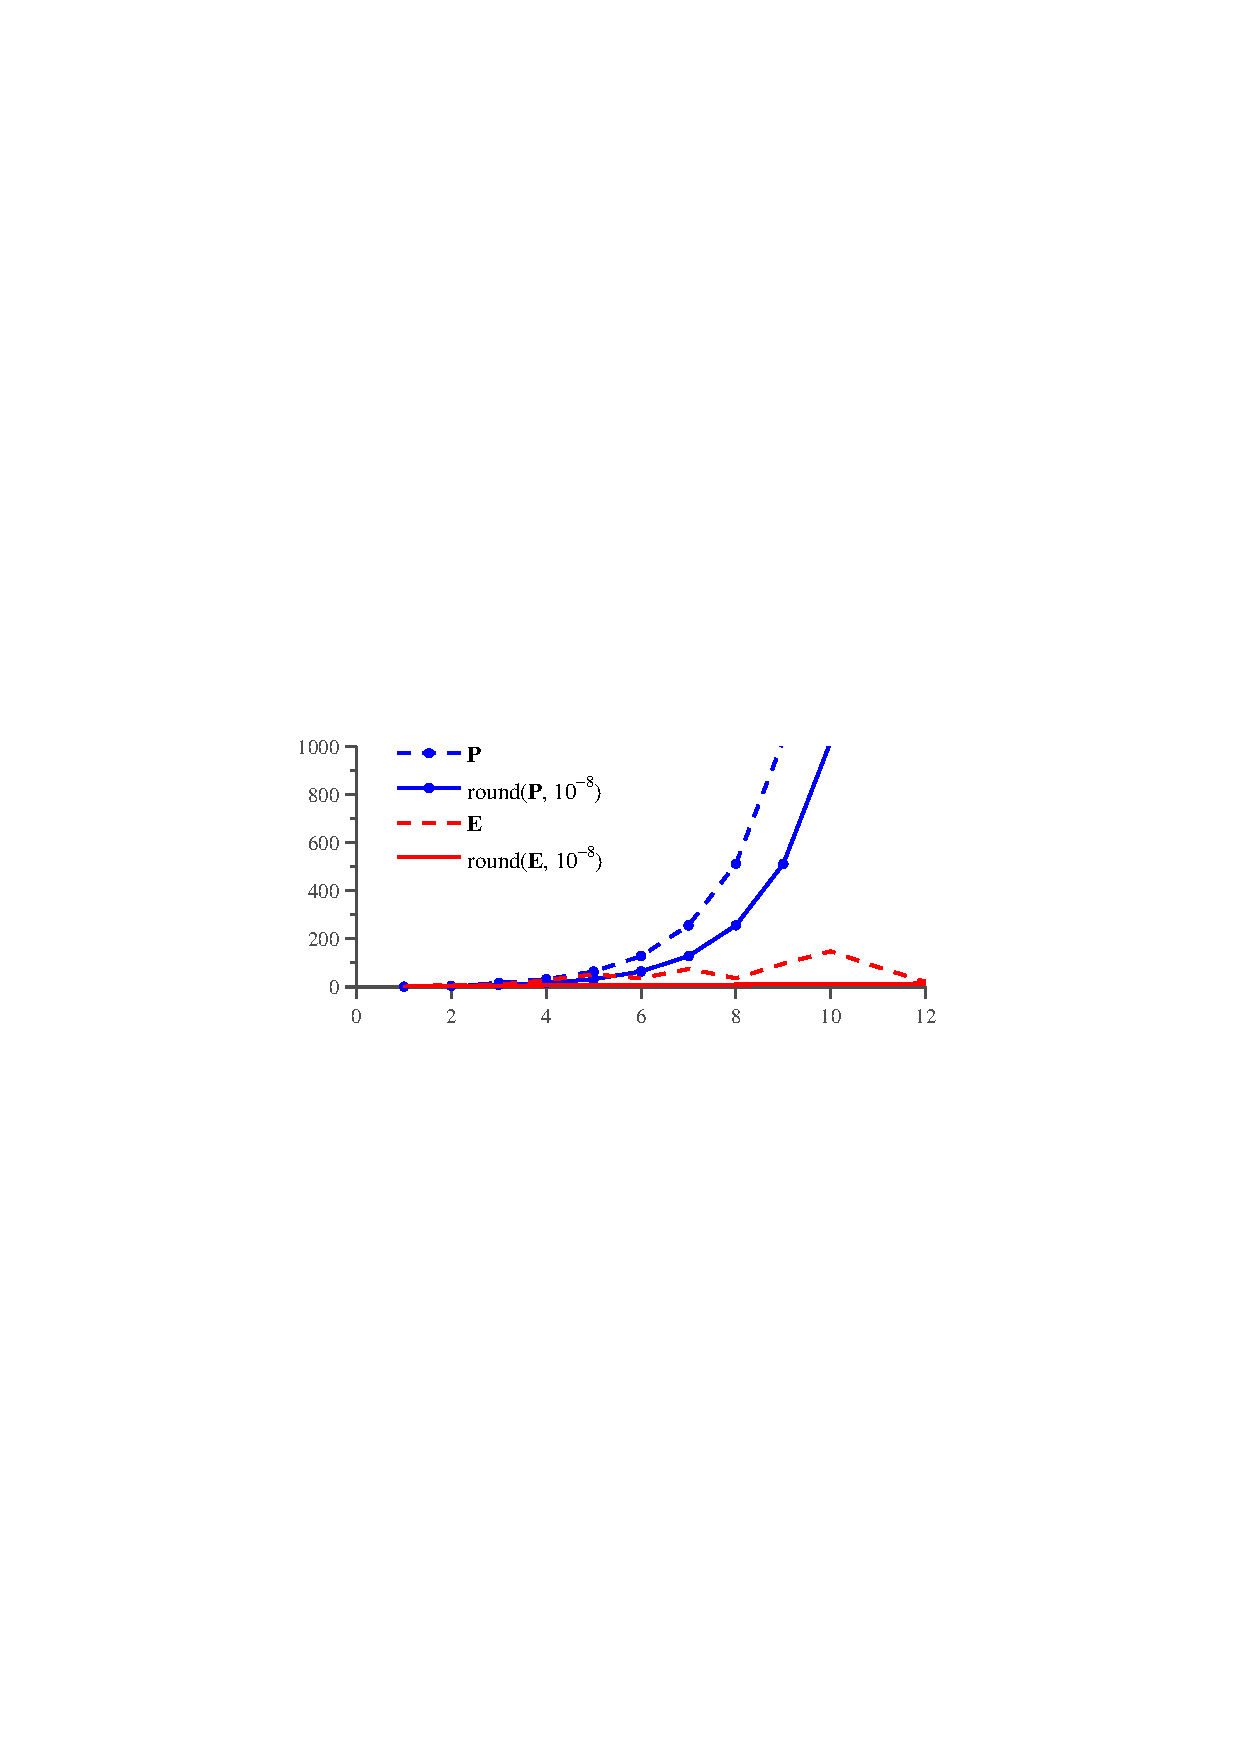
\includegraphics[width=7.0cm]{images/ranks_growth_temp=10,N=12,J=1_v2.pdf}
\\
& \parbox{7.3cm}{\centering\scriptsize размер решетки Изинга } \\
\end{tabular}
\caption{Максимальный TT\hyp{}ранг тензора энергии~$\mathbf{E}$ и тензора ненормированной вероятности~$\widehat{\mathbf{P}}$ для гомогенной решетки Изинга с температурой равной~10 и весами парных потенциалов равными~$1$. Детали см. в разделе \ref{sec::exp1}. \label{fig:ranks-growth}}
\end{center}
\end{figure}

\begin{figure}
\begin{center}
\begin{tabular}{m{0.3cm}@{}m{7cm}}
\begin{sideways}
\parbox{4cm}{\centering\scriptsize   }
\end{sideways}
& 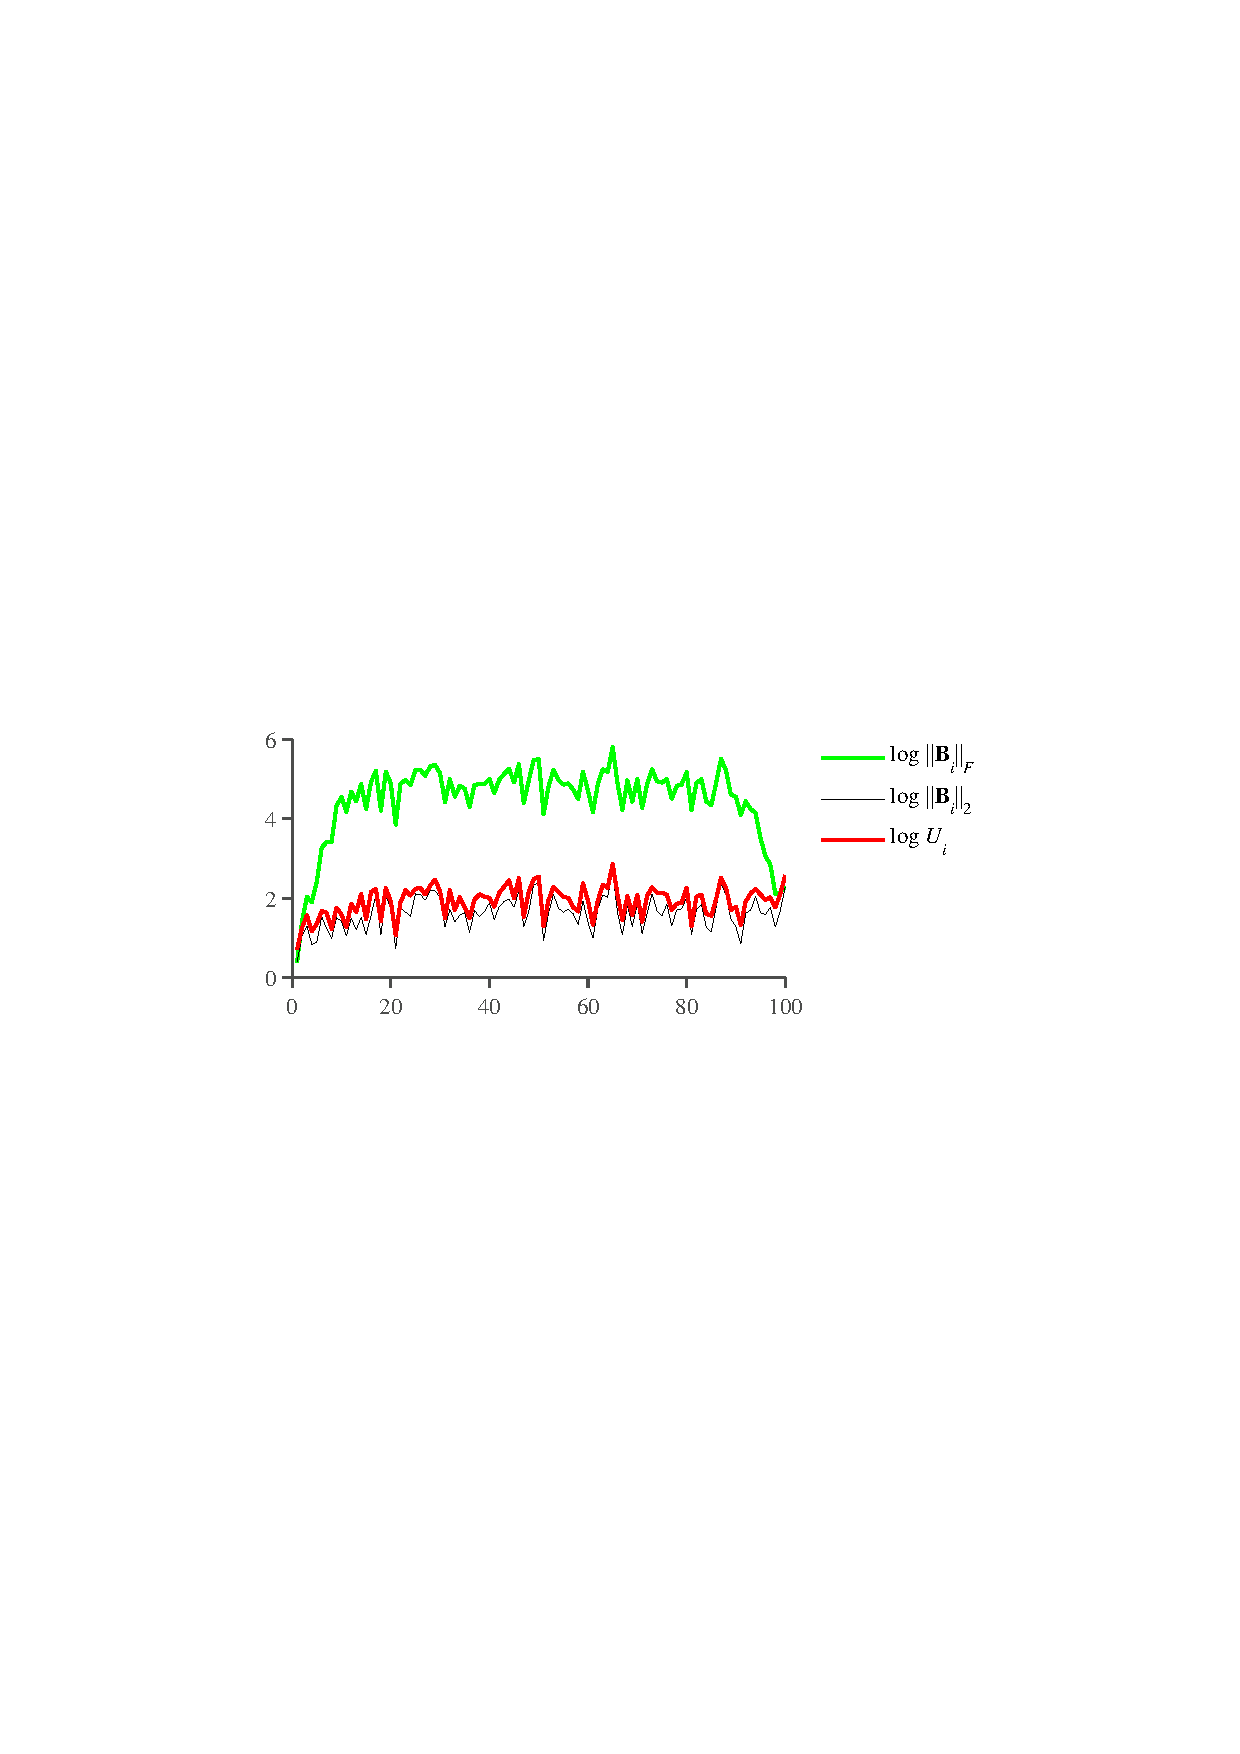
\includegraphics[width=7cm]{images/2norm.pdf}
\\
& \parbox{5.3cm}{\centering\scriptsize номер переменной~$i=1,\ldots,n$ } \\
\end{tabular}
\end{center}
\caption{ Сравнение Фробениусовой и спектральной нормы матрицы~$B_i$ с верхней оценкой~$U_i$. График построен для модели Изинга с решеткой размера $10 \times 10$, в которой коэффициенты унарных и парных потенциалов сгенерированы из равномерного распределения на $[-1, 1]$, а температура равна~$1$.
\label{fig:zUpperBound}}
\end{figure}
\begin{figure}
\begin{center}
\begin{tabular}{m{0.3cm}@{}m{7cm}}
\begin{sideways}\parbox{4cm}{\centering\scriptsize  $\log Z$ }\end{sideways}
& \includegraphics[width=7cm]{images/10x10,J=1,average=10,confInt_v3.pdf}
\\
& \parbox{7.3cm}{\centering\scriptsize температура~$T$} \\
\end{tabular}
\end{center}
\caption{Доверительный интервал на значение нормировочной константы~$Z$, полученный из теоремы~\ref{main-theorem} и неравенства~\eqref{eq:l2computing}. Детали см. в разделе \ref{sec::expZ}.  \label{fig:zConf}}
\end{figure}


\begin{figure}
\begin{center}
\begin{tabular}{m{0.3cm}@{}m{7cm}}
\begin{sideways}\parbox{4cm}{\centering\scriptsize  $\log Z$ }\end{sideways}
& \includegraphics[width=7cm]{images/10x10,J=1,average=10,confInt_v3.pdf}
\\
& \parbox{7.3cm}{\centering\scriptsize температура~$T$} \\
\end{tabular}
\end{center}
\caption{Доверительный интервал на значение нормировочной константы~$Z$, полученный из теоремы~\ref{main-theorem} и неравенства~\eqref{eq:l2computing}. Детали см. в разделе \ref{sec::expZ}.  \label{fig:zConf}}
\end{figure}

\begin{figure*}
\begin{center}
\vskip -0.3cm
\begin{tabular}{c@{}c@{\quad}c}
\begin{tabular}{m{0.3cm}@{}m{5.5cm}}
\begin{sideways}\parbox{4cm}{\centering\scriptsize  $|\log \widehat{Z} - \log Z|$ }\end{sideways}
& \includegraphics[width=5.5cm]{images/10x10,J=1,average=50_warm_MCMC_comparison_v3.pdf}
\\
& \parbox{5.8cm}{\centering\scriptsize температура~$T$ }
\label{fig:tmp}
\end{tabular}
&
\begin{tabular}{m{0.3cm}@{}m{5.5cm}}
\begin{sideways}\parbox{4cm}{\centering\scriptsize  $|\log \widehat{Z} - \log Z|$ }\end{sideways}
& \includegraphics[width=5.5cm]{images/wish_grid_mixed_n10_f1_0_worked3.pdf}
\\
& \parbox{5.8cm}{\centering\scriptsize сила парных потенциалов~$f$ }
\end{tabular}
&
% \includegraphics[width=1.8cm]{images/Z_legend_worked3.pdf}
\\
(a)
&
(b)
&
\\
\end{tabular}
\end{center}
\caption{На графиках представлены результаты экспериментов по подсчету нормировочной константы~$Z$. На графике~(a) предложенный метод (TT) сравнивается с другими на гомогенных моделях Изинга разной температуры. Для каждого значения температуры генерируется  50 моделей и указывается медиана и верхняя и нижняя квартили. На графике~(b) предложенный метод сравнивается с методом WISH на гетерогенных моделях Изинга. На обоих графиках изображены ошибки оценки~$Z$ (чем меньше значение --- тем лучше).
\label{fig:zExperiments}}
\end{figure*}



\alert{TODO: реализация.}


\subsection{Модель Изинга}
Основная модель для экспериментов --- \emph{модель Изинга}.
Функция энергии модели Изинга задаётся следующим образом:
% In our experiments we use the Ising model as the main playground.
% The energy of the model is defined as follows:
\begin{equation}
\label{eq::ising}
\mathbf{E}(\vec{x}) = -\frac{1}{T}\left(\sum_{i=1}^n x_i h_i + \sum_{(i,j) \in \mathcal{E}} c_{ij} x_i x_j\right),
\end{equation}
где переменные $x_i$, $i = 1,\ldots,n$ принимают значения из множества~$\{-1, 1\}$. Коэффициенты~$h_i$ будем называть \emph{унарными весами}, коэффициенты~$c_{ij}$ --- \emph{парными весами}, а~$T$ --- \emph{температурой}. Парные связи зависят от выбранного множества ребер~$\mathcal{E}$. В большинстве экспериментов будет использоваться 4-связная решетка размера~$10 \times 10$. Будем называть модель \emph{гомогенной}, если все парные веса равны друг другу ($c_{ij} = c$), и \emph{гетерогенной} иначе.
% where variables $x_i$, $i = 1,\ldots,n$ take values from set~$\{-1, 1\}$.  We refer to coefficients~$h_i$ as unary weights, to~$c_{ij}$ as pairwise weights, and to parameter~$T$ as temperature. Pairwise connections between the variables are determined w.r.t. a graph of connectivity. We typically use square 4-connected grids of $10\times 10$ nodes. If all pairwise weights are equal ($c_{ij} = c$) we call the Ising model  homogeneous and heterogeneous otherwise.

% \vspace{-0.2cm} In all our experiments we use a non-optimized MATLAB implementation of our methods. For operations related to the TT-format we use the TT-Toolbox\footnote{\url{http://spring.inm.ras.ru/osel/download/tt22.zip}} implemented in MATLAB.
% In our evaluation we use mainly use homogeneous and heterogeneous Ising model and we refer to the suppl. material for the detailed descriptions of the experimental setup.\\[-0.8cm]

\subsection{TT\hyp{}ранги энергии и вероятности \label{sec::exp1}}
В данном эксперименте проверяется утверждение из разделов~\ref{sec:energy-representation} и~\ref{sec:prob-representation}: при увеличении количества переменных TT\hyp{}ранги тензора энергии растут медленно, а TT\hyp{}ранги тензора ненормированной вероятности --- экспоненциально быстро~(рис.~\ref{fig:ranks-growth}). Рассматривается последовательность моделей Изинга с 4-x связной решеткой возрастающих размеров: от $1 \times 1$ до $12 \times 12$. Унарные веса $h_i$ сгенерированы из равномерного распределения $U[-1, 1]$, все парные веса $c_{ij}$ равны 1, температура $T$ равна 10. Для моделей Изинга указан максимальный TT\hyp{}ранг энергии и ненормированной вероятности при точном TT\hyp{}представлении и после TT\hyp{}округления с точностью~$10^{-8}$. Для точного TT\hyp{}представления тензора вероятности модели Изинга с решеткой размера $11 \times 11$ не хватает $8$GB оперативной памяти.

% \vspace{-0.1cm} In this experiment we illustrate the claims made in sec.~\ref{sec:energy-representation} and~\ref{sec:prob-representation} about the TT-ranks of the energy and the unnormalized distribution tensors constructed for an MRF. In fig.~\ref{fig:ranks-growth} for each size of an Ising model we report the maximal TT-ranks of both the energy and the unnormalized probability represented in the TT-format exactly and after the TT-rounding procedure with accuracy~$10^{-8}$. As was claimed the TT-ranks are growing slowly with the increase of the size of the model for the energies as opposed to the probabilities. The exact TT-representations of the probability tensors of sizes~$11$ and~$12$ did not fit into 8GB of memory.\\[-0.8cm]

\subsection{Нормировочная константа \label{sec::expZ}}
В данном эксперименте исследуется алгоритм оценки нормировочной константы MRF~(алг.~\ref{alg:Z-computing}).
% \vspace{-0.2cm} In this experiment we evaluate algorithm~\ref{alg:Z-computing} for computing the partition functions of MRFs.

В первом эксперименте метод, основанный на TT\hyp{}разложении (TT), сравнивается со следующими методами из библиотеки LibDAI~\cite{mooij10libdai}: Belief Propagation (BP)~\cite{kschischang01bp}, Tree Expectation Propagation (TREEEP)~\cite{minka04treeep}, и методом Mean Field (MF)~\cite{wainwright08gm}. Так же проводится сравнение с методом annealed importance sampling method (AIS)~\cite{neal01ais} --- представителем методов MCMC. Результаты представлены на рис.~\ref{fig:zExperiments}a. Рассматривается набор моделей Изинга с 4-х связной решеткой размера $10 \times 10$, где унарные веса $h_i$ сгенерированы из равномерного распределения $U[-1, 1]$, все парные веса $c_{ij}$ равны 1, температура $T$ меняется в пределах от $10^{-1}$ до $10^{3}$. Для каждого значения температуры сгенерировано 50 моделей Изинга и указана медиана и верхняя и нижняя квартили абсолютной ошибки оценки логарифма нормировочной константы. Для метода AIS были выбраны параметры (1000 промежуточных распределений с выборкой размером 70), максимизирующие точность, достигнутую за 60 секунд. Для подсчета правильных ответов был использован метод junction tree~\cite{wainwright08gm}.

Во втором эксперименте проводится сравнение с недавно предложенным методом WISH на данных из оригинальной статьи Ермона и др.~\cite{ermon13wish}. Ермон рассматривал набор моделей Изинга с решеткой размера $10 \times 10$, унарными весами $h_i$ сгенерированными из равномерного распределения $U[-1, 1]$, температурой $T$ равной 1, и парными весами $c_{ij}$ сгенерированными из равномерного распределения $U[-f, f]$, где параметр $f$ меняется от $0.25$ до $3$. Результаты сравнения представлены на рис.~\ref{fig:zExperiments}b. Отметим, что метод WISH запускался на кластере и каждое вычислительное ядро работало не менее 15 минут. Наш неоптимизированый Matlab код работал не более 53 секунд на каждом примере (32 секунды в среднем).


На рис.~\ref{fig:zConf} изображен доверительный интервал, полученный путем оценивания результата теоремы~\ref{main-theorem} неравенством~\eqref{eq:l2computing}.


\begin{figure}
\begin{center}
\begin{tabular}{c@{\!\!\!}c}
\begin{tabular}{m{0.3cm}@{}m{6.5cm}}
\begin{sideways}\parbox{4cm}{\centering\scriptsize  ошибка подсчета маргинала }\end{sideways}
& \includegraphics[width=6.5cm]{images/strong_mixed_spinglass_50_marginals_comparison_v3.pdf}
\\
& \parbox[t][0.5cm][t]{6.8cm}{\centering\scriptsize сила парных потенциалов~$f$ }
\end{tabular}
&
\includegraphics[width=2.3cm]{images/legend_marginals_v3.pdf}
\end{tabular}
\end{center}
\caption{Ошибка подсчета маргинальных распределений на наборе гетерогенных моделей Изинга. На графике указана среднемодульная ошибка вероятности класса ``-1'', усредненная по всем вершинам. Для каждого значения~$f$ генерируется 50 моделей Изинга и указывается медиана и верхняя и нижняя квартили.
 \label{fig:marginals}}
\end{figure}

\subsection{Унарные маргинальные распределения \label{sec::expMarg}}
В этом разделе исследуется качество подсчета маргинальных распределений предлагаемым методом (TT). Метод сравнивается с Belief Propagation (BP)~\cite{kschischang01bp}, Tree Expectation Propagation (TREEEP)~\cite{minka04treeep},  Mean Field (MF)~\cite{wainwright08gm} и Gibbs sampling~\cite{wainwright08gm}, реализованными в библиотеке LibDAI (рис.~\ref{fig:marginals}). Рассматривается набор моделей Изинга с решеткой размера $10 \times 10$, унарными весами $h_i$ сгенерированными из равномерного распределения $U[-1, 1]$, температурой $T$ равной 1, и парными весами $c_{ij}$ сгенерированными из равномерного распределения $U[-f, f]$, где параметр $f$ меняется от $0$ до $3$. Для каждого значения параметра $f$ результаты усредняются по 50 моделям.
% \vspace{-0.2cm} In these experiments we evaluate the ability of our method to compute the marginal distributions.
% We compare our method (TT) against Belief Propagation (BP)~\cite{kschischang01bp}, Tree Expectation Propagation (TREEEP)~\cite{minka04treeep},  Mean Field (MF)~\cite{wainwright08gm}, and Gibbs sampling~\cite{wainwright08gm} all implemented in the LibDAI system. The results of the comparison are presented in fig.~\ref{fig:marginals}.\\[-0.8cm]
%
\begin{table}[t]
\caption{Относительные значения энергии, достигнутые методом минимизации энергии, основанном на TT\hyp{}разложении. За $0\%$ взята нижняя граница энергии полученная методом TRW-S, за $100\%$ --- значение прямой энергии TRW-S.
% The relative value of energy for MAP-inference method based on the TT-decomposition. The lower bound ontained by TRW-S is $0\%$, the energy of TRW-S primal solution is $100\%$.
\label{tbl:map}}
\vskip 0.15in
\begin{center}
\begin{small}
%\begin{sc}
\begin{tabular}{lcccr}
\hline
%\abovespace\belowspace
Задача & $n$ & $d$ & Энергия TT  \\
\hline
%\abovespace
geo-surf-3/gm6   & 320 & 3 & 48.41\% \\
geo-surf-3/gm20 & 348 & 3 & 95.83\%  \\
geo-surf-3/gm203    & 187 & 3 & 98.69\%  \\
geo-surf-7/gm11   & 125 & 7 & 1769.65\%  \\
%\belowspace
matching/matching1    & 19 & 19 & 135.47\%   \\
\hline
\end{tabular}
%\end{sc}
\end{small}
\end{center}
\vskip -0.1in
\end{table}

\subsection{Минимизация энергии}
В данном эксперименте исследуется алгоритм минимизации энергии основанный на поиске минимального элемента тензора~$\mathbf{E}$. Для поиска минимального элемента тензора, представленного в TT\hyp{}формате, строится диагональная матрица в TT\hyp{}формате которая содержит все элементы исходного тензора на своей диагонали. Затем используется DMRG алгоритм Хоромского и Оселедца~\cite{khoromskij2010dmrg} для поиска минимального собственного значения TT\hyp{}матрицы. Данный метод сравнивается с популярным алгоритмом TRW-S~\cite{kolmogorov06trws} на реальных задачах из бенчмарка OpenGM~\cite{Kappes13comparison}. Часть результатов представлена в таблице~\ref{tbl:map}. Качество алгоритма DMRG сравнимо с качеством TRW-S и существенно выше на большинстве задач из раздела geo-surf-3. Более эффективные алгоритмы минимизации энергии ещё предстоит разработать.
% \vspace{-0.2cm} In this experiment we evaluate the algorithm of the search of the minimum element in an energy tensor which corresponds to MAP-inference. To find the minimum element of a tensor in the TT-format we construct a diagonal matrix in the TT-format containing all elements of the tensor and use the DMRG algorithm to find its minimal eigenvalue~\cite{khoromskij2010dmrg}. We run the method on several real-world tasks form a recent benchmark~\cite{Kappes13comparison} and compare it against the popular TRW-S algorithm~\cite{kolmogorov06trws}. Some of the results are reported in table~\ref{tbl:map}. The DMRG algorithm shows comparable results and on geo-surf-3 problems almost uniformly outperforms TRW-S.
% More efficient MAP-inference methods are yet to be developed.\\[-0.8cm]

\section{Реализация алгоритма сжатия нейросетей} \label{sec:exm-code}
Instead of compressing existing architectures one can use low-rank methods to be able to use much wider hidden layer than was available before. A recent work \cite{Jimmy2014lowRankSNN} shows that it is possible to construct wide and shallow neural networks with performance close to the state-of-the-art deep convolutional neural networks by training a shallow network on the outputs of a trained deep network. They report the improvement of performance with the increase of the hidden layer size and used up to $30\,000$ hidden neurons while restricting the matrix rank of the weight matrix in order to be able able to keep and to update it during the training. Restricting the TT-ranks of the weight matrix allows to use much wider layers that can potentially lead to greater expressive power of the model and we demonstrate it by outperforming other non-convolutional networks on the CIFAR-10 dataset by using several hundreds of thousands of hidden neurons.

\subsection{Свойства ТТ-слоя \label{sec:mnist-shapes}}

В данном эксперименте исследуются свойства ТТ-слоя и сравниваются различиные способы установки его параметра, таких как размерность тензоров представляющих вход и выход ТТ-слоя и ТТ-ранги факторизованной матрицы слоя. Данный эксперимент проводится на датасете распознавания рукописных цифр MNIST~\cite{lecun1998mnist}. Для увеличения количества возможных способов которыми можно представить входную картинку (исходный размер которой $28 \times 28$) в виде многомерного тензора изображения были перемасштабированы в разрешение $32 \times 32$. Для сравнения использовалась нейросеть с одним скрытым слоем нейронов размера 1024 и нелинейностью вида ReLU~\cite{RELU}. Данная сеть достигает тестовой ошибки  $1.9\%$ ($1.6\%$ при обучении с использованием техники дропаут~\cite{dropout}).

Для сравнения были обучены несколько сетей следующей архитектуры: ТТ-слой размера $1024 \times 1024$, нелинейность вида ReLU, полносвязный слой размера $1024 \times 10$. В качестве альтернативного метода сжатия рассматриалась нейросеть в которой вместо ТТ-слоя использовался полносвязный слой матрица которого представлялась и обучалась в низкоранговом формате. Для реализации данного бейзлайна использовалась сеть следующей архитектуры: полносвязный слой размера $1024 \times \rank$ (где $\rank$ это гиперпараметр обозначающий ранг низкорангового формата), полносвязный слой размера $\rank \times 1024$, нелинейность вида ReLU, полносвязный слой размера $1024 \times 10$. Результат данного эксперимента показана на Рис.~\ref{fig:mnist-shape}. Из представленного графика следует, что ТТ-разложение позволяет добиться существенно большего уровня сжатия чем сжатие через низкоранговое разложение при той же точности, и предоставляет больший диапазон выбора баланса между сжатием и точностью.



\begin{figure}[t]
  \begin{center}
  \setlength\figureheight{5.2cm}
  \setlength\figurewidth{9cm}
  % This file was created by matlab2tikz v0.4.7 running on MATLAB 8.1.
% Copyright (c) 2008--2014, Nico Schlömer <nico.schloemer@gmail.com>
% All rights reserved.
% Minimal pgfplots version: 1.3
%
% The latest updates can be retrieved from
%   http://www.mathworks.com/matlabcentral/fileexchange/22022-matlab2tikz
% where you can also make suggestions and rate matlab2tikz.
%
%
% defining custom colors
\definecolor{mycolor1}{rgb}{0.00000,0.00000,0.17241}%
\definecolor{mycolor2}{rgb}{1.00000,0.10345,0.72414}%
\definecolor{mycolor3}{rgb}{0.00000,0.34483,0.00000}%
%
\begin{tikzpicture}

\begin{axis}[%
width=\figurewidth,
height=\figureheight,
scale only axis,
xmode=log,
xmin=20,
xmax=2500000,
xminorticks=true,
xlabel={число параметров в матрице первого слоя},
ymode=log,
ymin=1,
ymax=100,
yminorticks=true,
ylabel={тестовая ошибка \%},
axis x line*=bottom,
axis y line*=left,
legend style={draw=none,fill=white,legend cell align=left,at={(1.6,1)},anchor=north east}
]
\addplot [color=blue,solid]
  table[row sep=crcr]{2048  2.15\\
4096    3.38\\
6144    3.41\\
8192    3.27\\
};
\addlegendentry{$32 \times 32$};

\addplot [color=red,solid]
  table[row sep=crcr]{160   2.77\\
576 1.64\\
1248    1.63\\
2176    1.6\\
};
\addlegendentry{$4 \times 8 \times 8 \times 4$};

\addplot [color=green,solid]
  table[row sep=crcr]{80    2.7\\
256 2.42\\
528 1.75\\
896 1.7\\
};
\addlegendentry{$4 \times 4 \times 4 \times 4 \times 4$};

\addplot [color=mycolor1,solid]
  table[row sep=crcr]{144   3.03\\
560 2.03\\
1248    2.1\\
2208    1.74\\
};
\addlegendentry{$2 \times 2 \times 8 \times 8 \times 2 \times 2$};

\addplot [color=mycolor2,solid]
  table[row sep=crcr]{40    3.35\\
144 2.87\\
312 2.29\\
544 2.11\\
};
\addlegendentry{$2^{10}$};

\addplot [color=mycolor3,dashed]
  table[row sep=crcr]{2048  66.89\\
20480   3.54\\
102400  2.29\\
204800  2.24\\
};
\addlegendentry{матричный низкоранговый формат};


\addplot [only marks,color=black,solid,mark=*,mark options={solid},mark size=1.5pt]
  table[row sep=crcr]{1000000 1.9\\
};
\addlegendentry{несжатый слой};


\end{axis}
\end{tikzpicture}%

  \end{center}
  \caption{Экспериментальное сравнение свойст сжатия нейросетей при помощи ТТ-разложения на датасете MNIST. На оси Y отложена тестовая ошибка, на оси X число параметров первого слоя нейросети (число элементов ТТ-ядер в случае ТТ-слоя и $2048  \rank$ в случае низкорангового сжатия). Каждая кривая соответсвующая ТТ-разложению отвечает одному из способов представить входной и выходной вектор ТТ-слоя в виде многомерного массива. Числа разеделенные символов  ``$\times$'' обозначает арности каждой из размерностей тензоров входа и выхода. Различные точки принадлижащие одной кривой отличаются ТТ-рангами и матричными рангами соответсвенно. количество параметров в исходном (несжатом) слое равно~$10^6$. \label{fig:mnist-shape}}
\end{figure}


 \subsubsection{Сравнения порядков элементов во входных данных}
В данном эксперименте сравнивается обучения нейросети с ТТ-слоем на исходных данных датасета MNIST с обучением аналогичной нейросети на данных в которых все пиксели входных картинок случайно перемешаны (при этом случайная перестановка зафиксирована и не меняется во время обучения и тестирования). Используется нейросеть со следующей архитектурой: ТТ-слой размера $1024 \times 15\,625$ и TT-рангом 2, нелинейность вида ReLU, полносвязный слой размера $15\,625 \times 10$. Обучение на исходных данных приводит к тестовой ошибке $1.6$, тогда как обучение на данных после применения случайной перестановки приводит к тестовой ошибке $2.6$. Таким образом, эффективного сжатия ТТ-формат достигает благодаря использования структуры входных данных, которая разрушается при перемешивании порядка пикселей во входной тензоре.


\paragraph{Сравнение с работой HashedNet~\cite{chen2015compressing}.} В данном эксперименте рассматривается нейронная сеть с одним скрытым слоем размера $1024$ нейрона в которой оба полносвязных слоя заменяются ТТ-слоями. При установки всех ТТ-рангов в сети в значение 8 была достигнута тестовая ошибка $1.6\%$ при использовании $11\,210$ параметров во всей сети. При установлении ТТ-рангов в значение 6 была досигнута тестовая ошибка $1.9\%$ с использованием $6\,842$ параметров. В работе~\cite{chen2015compressing} при использовании такой же архитектуры были достигнуты следующие результаты при помощи связывания случайных подмножеств весов: сжатие сети в $64$ раза до  $12\,422$ параметров при достижении тестовой ошибки $2.79\%$.\\

\subsection{CIFAR-10}
Датасет CIFAR-10~\cite{krizhevsky2009Cifar} состоит из цветных изображений размера $32 \times 32$ каждому из которых присвоены один из 10 классов: аэроплан, автомобиль, птица, кошка, олень, собака, лягушка, лошадь, корабль, грузовик. Датасет состоит из  50000 обучающих и 10000 тестовых изображений. Во всех последующих экспериментах в качестве предобработки изображений из них вычитается среднее, выполняется нормализация конраста и предобразования ZCA так же как описано в работе~\cite{goodfellow2013maxout}.

% \subsubsection{Compression}
Для экспериментов была выбрана сверточная нейронная сеть CIFAR-10 Quick~\cite{snoek2012cifarQuick} состоящия из сверточного слоя, пулинга и нелийности за которыми следуют два полносвязных слоя с нейлинейностями размера  $1024 \times 64$ и $64 \times 10$. Сверточная часть сети в эксперименте была зафиксирована, а полносвязная часть заменена ТТ-слоем размера $1024 \times N$, нелинейностью типа ReLU и полносвязного слоя размера $N \times 10$. Используя $N = 3125$ скрытых нейронов (в исходной сети использовалось $64$) было достигнуто тестовая ошибка $23.13\%$ без дообучения, что превосходит аналогичный показатель исходной сети ($23.25\%$ ошибки). Тензорная размерность входного вектора использовалась $4 \times 4 \times 4 \times 4 \times 4$, а выходного вектора $5 \times 5 \times 5 \times 5 \times 5$. При фиксировании ТТ-рангов в значение 8 ТТ-слой обладает $4160$ настраиваемым параметрам, что соотсвтесвует сжатию всей сети по сравнению с исходной сетью в $1.24$ раза. При замене обоих полносвязных слоев на ТТ-слои доводит тестовую ошибку до $24.39\%$ и приводит к сжатию полносвязной части сети в $11.9$ раз и сжатию всей сети в $1.7$ раз.

Для сравнения, в работе~\cite{Denil2013predicting} полносвязные слои сверточной сети для датасета CIFAR-10 были сжаты не более чем в $4.7$ раз при потере $2\%$ точности.

\subsubsection{Широкая и неглубокая сеть}
Согласно теореме из работы~\cite{cybenko1989universalApproximator}, нейросети являются универсальными аппроксиматорами, т.е. при достаточном количестве скрытых нейронов нейросеть с одним скрытым слоем способна приблизить любую непрерывную решающую границу. Обычно сети достаточно широкие чтобы подойти к границы применимости данной теоремы не используются на практике, так как требует высоких вычислительных затрат, большого объема памяти и могут приводить к переобучению из-за слишком большого количества настраиваемых параметров. Использование широких ТТ-слоев потенциально может исправить все три озвученные проблемы. В данном эксперименте используется нейросеть с двумя скрытыми слоями следующей архитектуры: ТТ-слой размера $3072 \times 262\,144$, нелинейность типа ReLU, ТТ-слой размера $262\,144 \times 4\,096$, нелинейность типа ReLU, полносвязный слой размера $4\,096 \times 10$. Такая нейронная сеть достигает тестовой ошибки в $31.47\%$, что делает ее одной из лучших в классе полносвязных сетей для датасета CIFAR-10.

\begin{table}
    \begin{center}
    \begin{tabular}{ l@{\;}|@{\;}c@{\;}|@{\;}c@{\;}|@{\;}c@{\;}|@{\;}c@{\;}|@{\;}c@{\;}|@{\;}c@{\;}|@{\;}c@{\;} }
    % \hline
    Архитектура &
    \parbox{2cm}{Сжатие \\ ТТ-слоев} &
    \parbox{1.5cm}{Cжатие \\ vgg-16} &
    \parbox{1.5cm}{Cжатие \\ vgg-19} &
    \parbox{1.5cm}{Топ 1 \\ vgg-16} &
    \parbox{1.5cm}{Топ 5 \\ vgg-16} &
    \parbox{1.5cm}{Топ 1 \\ vgg-19} &
    \parbox{1.5cm}{Топ 5 \\ vgg-16} \rule{0pt}{1.0\normalbaselineskip} \\ \hline
    FC FC FC \rule{0pt}{1.0\normalbaselineskip}     & $1$ &  $1$ & $1.0$ & $30.9$ &  $11.2$ & $29.0$ & $10.1$  \\ % \hline
    TT4 FC FC    & $50\,972$ & $3.9$ & $3.5$ & $31.2$ & $11.2$ & $29.8$ & $10.4$ \\ % \hline % 2016 params vs 25088 \times 4096
    TT2 FC FC    & $194\,622$ & $3.9$ & --  & $31.5$ & $11.5$ & -- & -- \\ % \hline % 528 params vs 25088 \times 4096
    TT1 FC FC    & $713\,614$ & $3.9$ & --  & $33.3$ & $12.8$ & -- & -- \\ % \hline % 144 params vs 25088 \times 4096
    TT4 TT4 FC    & $37\,732$ & $7.4$ & -- & $32.2$ & $12.3$ & -- & -- \\ % \hline % 1152 params vs 4096 \times 4096
    LR1 FC FC    & $3\,521$ & $3.9$ & -- & $99.5$ & $97.6$ & -- & -- \\ % \hline % 1152 params vs 4096 \times 4096
    LR5 FC FC    & $704$ & $3.9$ & $3.5$ & $81.7$ & $53.9$ & $79.1$ & $52.4$ \\ % \hline % 1152 params vs 4096 \times 4096
    LR50 FC FC    & $70$ & $3.7$ & $3.4$ & $36.7$ & $14.9$ & $34.5$ & $15.8$ \\ % \hline % 1152 params vs 4096 \times 4096
    \end{tabular}
    \end{center}
    \caption{Сжатие полносвязных слоев сверточных сетей  vgg-16 и vgg-19 на датасете ImageNet. Каждая строчка означает архитектуру последних трех слоев сети, ``FC'' означает (несжатый) полносвязный слой; TT$\square$ означает ТТ-слой с ТТ-рангом равным числу  ``$\square$'' указанному рядом; LR$\square$ означает полносвязный слой с матрицей представленный в низкоранговом формате с рангом ``$\square$''. Во второй колонке указан уровень сжатия тех слоев которые сжимались в данной архитектуре, в третей и четвертой колонке сжатие всей сети. В колонках номер 5-8 указаны топ 1 ошибка (ошибка классификации) и топ 5 ошибка (количество тестовых примерых на которых правильный ответ попал в первые 5 кандидатов предложенных нейросетью) \label{tbl:imagenet-vgg-layer}}
\end{table}
% Convolutional part params: 14714688 in vgg-16, 20024384 in vgg-19
% fc part: 123642856

\subsection{ImageNet}
В данном эксперименте исследуется способность ТТ-слоя к сжатию нейросетей обученных на больших объемах данных. Рассматривается датасет ImageNet ILSVRC-2012 dataset~\cite{Russakovsky2015ImageNet} который состоит из 1.2 миллиона обучающих изображений и 50000 валидационных изображений, каждое из которых отнесено к одному из 1000 классов. В качестве базовых моделей используются сверточные нейросети vgg-16 и vgg-19~\cite{simonyan15}. Обе нейросети состоят из двух частей: сверточной и полносвязной. В обоих сетях полносвязныя часть состоит из трех полносвязных слоев размеров $25088 \times 4096$, $4096 \times 4096$ и $4096 \times 1000$.

Сначала, в обоих сетях первый полносвязный слой был заменен на ТТ-слой у которого входной вектор длины $25088$ был преобразован в тензор размера $2 \times 7 \times 8 \times 8 \times 7 \times 4$, а выходной вектор длины $4096$ был преобразован в тензор размера $4 \times 4 \times 4 \times 4 \times 4 \times 4$. Оставшиеся два полносвязных слоя были случайно переинициализорваны и обучены с нуля. Параметры сверточной части сетей были зафиксированы во время обучения в значения найденные в работе~\cite{Russakovsky2015ImageNet}. Ошибка на валидационном множестве и сжатия относительно исходной версии сетей для разных значений ТТ-рангов приведены в Тбл.~\ref{tbl:imagenet-vgg-layer}. При использовании ТТ-ранга 2 это приводит к сжатию матрицы самого большого полносвязного слоя сети в $194\,622$ раз ($25088 \times 4096$ параметров в исходной матрице и $528$ параметров в ТТ-матрице) и при этом увеличить топ 5 ошибку сети с $11.2$ до $11.5$. Это приводит к сжатию всей сети в 3.9 раз. В следующем эксперименте сжатию подвергаются также и второй полносвязный слой сетей, что приводит к сжатию всей сети в 7.4 раза.

В качестве бейзлайна рассматривается сжатие первого полносвязного слоя при помощи ограничения матричного ранга матрицы слоя~\cite{Jimmy2014lowRankSNN}, что приводит к существенному снижению точности даже при использовании относительно высокого ранга 50 (ошибка увеличивается с 11.2 до 14.9). В другом методе сжатия нейросетей~\cite{yang2014deep} было получено сжатие сети в 2-3 раза без увеличения ошибка классификации, однако в их работе использовалась другая архитектура базовой сети~\cite{Krizhevsky2012AlexNet}, так что результаты не сравнимы напрямую.




% \begin{table}
%     \begin{center}
%     \begin{tabular}{ l | l | l | l | l | l}
%     % \hline
%     Model & fc part compression & whole compression & error before & error after & relative difference \rule{0pt}{1.0\normalbaselineskip}\\ \hline
%     Fastfood-16-AD & $3.6$ & $3.6$ & $42.59\%$ & $45.30\%$ & $+6.4\%$ \rule{0pt}{1.0\normalbaselineskip} \\ % \hline
%     Fastfood-32-AD & $1.8$ & $1.8$ & $42.59\%$ & $43.77\%$ & $+2.8\%$ \\ % \hline
%     Fastfood-16-AD + finetuning & $3.6$ & $3.6$ & $42.59\%$ & $42.90\%$ & $+0.7\%$ \\ % \hline
%     Fastfood-32-AD + finetuning & $1.8$ & $1.8$ & $42.59\%$ & $41.93\%$ & $-1.5\%$ \\ % \hline
%     tt4 fc fc & $5.9$ & $3.9$ & $30.9\%$ & $31.2\%$ & $+1\%$ \\ % \hline
%     tt4 tt4 fc & $\boldsymbol{30}$ & $\boldsymbol{7.4}$ & $30.9\%$ & $32.2\%$ & $+4.2\%$ \\ % \hline
%     \end{tabular}
%     \end{center}
%     \caption{Comparison with Fastfood networks~\cite{yang2014deep}. The reference convnet of the Fastfood method contains more than $99.9\%$ of parameters in the fully-connected part, so for their model the compression rates for the fully-connected part and for the whole network are roughly the same.\label{tbl:fastfood}}
% \end{table}


% On the forward pass the TT-layer is up to $13$ times faster than the fully-connected analog~(Table~\ref{tbl:imegenet-inference}). Note that the TT code is written in MATLAB while the fully-connected layer is implemented in C and CUDA.
\begin{table}
    \begin{center}
    \begin{tabular}{l| l l}
    Type & 1 im. time (s$/100$) & 100 im. time (s$/100$) \rule{0pt}{1.0\normalbaselineskip}\\ \hline
    CPU fully-connected layer   & $1.609$ & $9.72$ \rule{0pt}{1.0\normalbaselineskip}\\
    CPU TT-layer   & $0.124$ & $9.47$\\
    GPU fully-connected layer   & $0.27$ & $3.3$\\
    GPU TT-layer   & $0.192$ & $1.286$\\
    \hline
    CPU fully-connected layer   & $4.1$ & $4.9$ \rule{0pt}{1.0\normalbaselineskip}\\
    CPU TT-layer   & $0.19$ & $6.1$\\
    GPU fully-connected layer   & $0.08$ & $0.4$\\
    GPU TT-layer   & $0.04$ & $0.4$\\
    \end{tabular}
    \end{center}
    \caption{Inference time for the $25088 \times 4096$ fully-connected layer and its corresponding TT-layer with all the TT-ranks equal $4$. The memory usage for feeding forward one image is $392$MB for the fully-connected layer and $0.766$MB for the TT-layer. \label{tbl:imegenet-inference} \vspace{-0.5cm}}
\end{table}
% CPU:
% TT small: 0.001226 0.001240 0.001258, mean 0.001243 +- 0.000020
% Conv small: 0.016052 0.016072 0.016109, mean 0.016094 +- 0.000077
% FC small: 0.111983 0.112402 0.112718, mean 0.112417 +- 0.000563
% TT big: 0.094254 0.094626 0.094908, mean 0.094658 +- 0.000527
% Conv big: 0.096744 0.097039 0.097399, mean 0.097159 +- 0.000791
% FC big: 0.197489 0.197676 0.198054, mean 0.197895 +- 0.000838
% GPU:
% TT small: 0.001912 0.001916 0.001923, mean 0.001924 +- 0.000047
% Conv small: 0.002680 0.002684 0.002690, mean 0.002697 +- 0.000124
% FC small: 0.009794 0.009796 0.009801, mean 0.009802 +- 0.000052
% TT big: 0.012849 0.012854 0.012860, mean 0.012863 +- 0.000081
% Conv big: 0.032895 0.032934 0.033011, mean 0.032957 +- 0.000124
% FC big: 0.035456 0.035477 0.035502, mean 0.035482 +- 0.000037




% TODO: say what was the learning procedure? weight decay, learning rate, momentum, etc

% Multiplying one TT-core by a positive constant and dividing another TT-core by the same constant does not change the elements of matrix $\mat{W}$ (see eq.~\ref{eq:TT-layer-output-detailed}) leading to ambiguity in TT-representation.
We use L$2$-regularization term for the TT-cores elements with $\lambda = 0.0005$ to prevent ambiguities in the TT-format. To initialize all the parameters (the elements of the TT-cores for TT-layers and the weight matrices for fully-connected layers) we use Gaussian noise. We train TensorNets with stochastic gradient descent with momentum (with coefficient $0.9$) and tune the learning rate by hand on the validation set.


\section{Реализация тензорных полиномиальных моделей} \label{sec:exm-experiments}

%\begin{figure}
%    \centering
%    \begin{subfigure}[b]{\textwidth}
%        \includegraphics[width=\textwidth]{images/riemannian_vs_plain_car_train.pdf}
%        \caption{обучающая выборка}
%    \end{subfigure}
%    \begin{subfigure}[b]{\textwidth}
%        \includegraphics[width=\textwidth]{images/riemannian_vs_plain_car_validation.pdf}
%        \caption{валидационная выборка}
%    \end{subfigure}
%    \caption{Бинаризованный набор данных Car, сравнение стохастической римановой оптимизации с стохастическим градиентным спуском примененным к элементам ТТ-ядер для модели рекуррентной нейросети ТТ-ранга-$4$. Числа в легенде отражают размер мини-батча ($M$, число объектов использующихся на каждом шаге стохастической оптимизации). Графики отмеченные как `сл. иниц.' (квадратные  маркеры) отвечают запускам метода оптимизации со случайного ТТ-тензора ранга 4 (ядра которого заполнены стандартным нормальным шумом). \alert{todo: перевести легенду и выкинуть одну из инициализаций}.
%Все остальные кривые отвечают запускам инициализированным с решения линейной версии задачи (см. раздел~\ref{sec:exm-initialization}).}\label{fig:riemannian_vs_plain_car}
%\end{figure}



%\begin{figure}
%    \centering
%    \begin{subfigure}[b]{\textwidth}
%        \includegraphics[width=\textwidth]{images/riemannian_vs_plain_hiv_train.pdf}
%        \caption{обучающая выборка}
%    \end{subfigure}
%    \begin{subfigure}[b]{\textwidth}
%        \includegraphics[width=\textwidth]{images/riemannian_vs_plain_hiv_validation.pdf}
%        \caption{валидационная выборка}
%    \end{subfigure}
%    \caption{Набор данных HIV, сравнение стохастической римановой оптимизации с стохастическим градиентным спуском примененным к элементам ТТ-ядер для модели рекуррентной нейросети ТТ-ранга-$4$. Числа в легенде отражают размер мини-батча ($M$, число объектов использующихся на каждом шаге стохастической оптимизации). Графики отмеченные как `сл. иниц.' (квадратные  маркеры) отвечают запускам метода оптимизации со случайного ТТ-тензора ранга 4 (ядра которого заполнены стандартным нормальным шумом). \alert{todo: перевести легенду и выкинуть одну из инициализаций}.
%Все остальные кривые отвечают запускам инициализированным с решения линейной версии задачи (см. раздел~\ref{sec:exm-initialization}).}\label{fig:riemannian_vs_plain_hiv}
%\end{figure}

\subsection{Наборы данных \label{sec:exp-datasets}}
Наборы данных используемые в экспериментах $\alert{todo: compare with RNN wrt learning speed?}$
\begin{enumerate}
  \item Выборка \textbf{UCI~\cite{Lichman2013UCI} Car} это задача  классификации с $1728$ объектами и $21$ бинарными признаками (после превращения `one-hot' преобразование, которое заменяет категориальный признак который может принимать $K$ возможных значений на бинарный вектор длины $K$ такой что только один элемент этого вектора ненулевой в любом объекте).
  Данные были случайным образом разделены на  $1382$ обучающих  и $346$ валидационных объекта. Метки датасета были бинаризованы путем конвертации метки исходного первого класса в `0' и всех остальных классов в `1'.

  \item Выборка \textbf{UCI~\cite{Lichman2013UCI} HIV} это задача бинарной классификации с $1625$ объектами и $160$ признаками, которая была разбита на $1300$ обучающих и $325$ валидаионных объекта.

  \item \textbf{Сгенерированные данные.} Были сгенерированны $100\,000$ обучающих и $100\,000$ валидационных объекта с $30$ признаками.
  Каждый элемент матрицы объект-признак $X$ был независимо сгенерирован из равномерного распределения над $\{-1, +1\}$.
  Так же были случайно выбраны $20$ подмножеств признаков порядка 6 из равномерного распределения: $j^1_1, \ldots, j^1_{6}, \ldots, j^{20}_1, \ldots, j^{20}_{6} \sim \mathcal{U}\{1, \ldots, 30\}$.
  Целевой признак был установлен в детерминированную функцию входа: $y(\vec{x}) = \sum_{z=1}^{20} \varepsilon_z \prod_{h=1}^{6} x_{j^z_h}$, где веса мономов были сгенерированны из равномерного распределения: $\varepsilon_1, \ldots, \varepsilon_{20} \sim \mathcal{U}(-1, 1)$.

%  \item \textbf{MovieLens 100K.} MovieLens 100K это выборка данных рекомендательной системы в которой есть $943$ пользователей и $1\,682$ фильмов~\cite{harper2015movielens}.
%  Выборка была превращена в задачу бинарной классификации, а признаки были обработанны так же, как и в работе~\cite{blondel2016hofm}:
%  \begin{enumerate}
%  \item Для пользователей в качестве признаков использовался год округленный до десятилетий, район (первая цифра индекса), пол и занятость как категориальные признаки.
%  \item Для фильмов, в качестве признаков использовался год выхода на экран (округленный до десятилетий) и жанр.
%  \item Исходные рейтинги фильмов были бинаризованы по порогу $5$.
%  \end{enumerate}
%  Итоговая выборка после обработки состоит из $21\,200$ положительных примеров ("фильм понравился"), половина из которых использовалась для обучения вместе с равным количеством отрицательных примеров, а вторая половина для валидации.
\end{enumerate}


\subsection{Риманова оптимизация \label{sec:exp-riemannian-optimization}}
В данном эксперименте сравниваются два подхода к обучению модели~\eqref{eq:polynomial-model}: стохастическая риманова оптимизация (см. раздел~\ref{sec:exm-riemannian-optimization}) и стохастический градиентный спуск примененный к элементам ТТ-ядер. В обоих методах для выбора длины шага оптимизации возможные шаги перебирались по сетке и выбирался наилучший согласно качеству на обучающей выборке через 100 шагов оптимизации.

На выборках Car и HIV параметр регуляризации устанавливался $\lambda = 0$, а ТТ-ранг $r = 4$.
На выборке Car метод стохастической оптимизации (оптимальная длина шага для которого составила $\alpha = 40$) сходится быстрее и к лучшему значению функционала чем альтернативный метод (оптимальная длина шага для которого составила $\alpha = 0.03$) как с точки зрения обучающей, так и с точки зрения валидационной ошибки.~(Рис.~\ref{fig:riemannian_vs_plain_car}a,b).
На выборке HIV стохастическая риманова оптимизация  (с длиной шага $\alpha = 800$) сходится к значения функционала $10^{-4}$ в $20$ раз быстрее альтернативного метода оптимизации~(длина шага которого составила $\alpha = 0.001$, см Рис.~\ref{fig:riemannian_vs_plain_hiv}a), однако модель переобучается под данные~(Рис.~\ref{fig:riemannian_vs_plain_hiv}b).

На сгенерированной выборке обучить модель при помощи стохастического градиентного спуска не получилось ни при каком значении величины шага, тогда как стохастическая риманова оптимизация обучает данную модель~(Рис.~\ref{fig:riemannian-vs-plain-synthetic}).

%On the MovieLens 100K dataset, we have only used SGD-type algorithms, because using the one-hot feature encoding is much slower than using the categorical version (see Sec.~\ref{sec:model-extension}), and we have yet to implement the support for categorical features for the Riemannian optimizer.
%On the bright side, prototyping the categorical version of ExM in TensorFlow allowed us to use a GPU accelerator.
%
%
%\subsection{Initialization \label{sec:exp-initialization}}
%In this experiment, we compared random initialization with the initialization from the solution of the corresponding linear problem~(Sec.~\ref{sec:initialization}).
%We explored two ways to randomly initialize a TT-tensor: 1) filling its TT-cores with independent Gaussian noise; 2) initializing $\tens{W}$ to represent a linear model with random coefficients (sampled from a standard Gaussian).
%We report that on the Car dataset type-1 random initialization slowed the convergence compared to initialization from the linear model solution~(Fig.~\ref{fig:riemannian_vs_plain}a), while on the HIV dataset the convergence was completely frozen in case of the type-1 initialization~(see Fig.~\ref{fig:riemannian_vs_plain}b).
%
%Two possible reasons for this effect are:
%a) the vanishing and exploding gradients problem~\cite{bengio1994vanishing} that arises when dealing with a product of a large number of factors ($160$ in the case of the HIV dataset);
%b) by initializing the model in such a way that high-order terms dominate we may force the gradient-based optimization to focus on high-order terms at the beginning, while it may be beneficial to start with determining low-order terms instead.
%
%Type-2 initialization (a random linear model) worked on par with initialization from the solution of the linear problem on the Car, HIV, and synthetic datasets~(Fig.~\ref{fig:riemannian_vs_plain_car},~\ref{fig:riemannian_vs_plain_hiv},~\ref{fig:riemannian-vs-plain-synthetic}).
%This may indicate that the problem with type-1 initialization is indeed not in the randomness per se, but in giving too much attention to high-order terms at the beginning of the optimization process.
%
%
%\subsection{Comparison to other approaches \label{sec:exp-comparison}}
%On the synthetic dataset with high-order interactions we compared Exponential Machines (the proposed method) with scikit-learn implementation~\cite{scikit-learn} of logistic regression, random forest, and kernel SVM; FastFM implementation~\cite{bayer2015fastfm} of $2$-nd order Factorization Machines; our implementation of high-order Factorization Machines\footnote{\url{https://github.com/anonymized}}; and a feed-forward neural network implemented in TensorFlow~\cite{tensorflow2015-whitepaper}.
%We used $6$-th order FM with the Adam optimizer~\cite{kingma2014adam} for which we had chosen the best rank ($20$) and learning rate ($0.003$) based on the training loss after the first $50$ iterations.
%We tried several feed-forward neural networks with ReLU activations and up to $4$ fully-connected layers and $128$ hidden units.
%We compared the models based on the Area Under the Curve (AUC) metric since it is applicable to all methods and is robust to unbalanced labels.
%We report that our model works on par with high-order Factorization Machines and outperforms all the baselines in the case of limited training time budget (yielding $0.85$ test AUC in 1831 seconds, see Tbl.~\ref{tbl:synthetic-comparison}).
%
\begin{table}[t]
\caption{Сравнение различных методов классификации на сгенерированных данных (см. раздел~\ref{sec:exp-comparison}).
Во второй колонке приведена мера качества AUC (площадь под РОК-кривой), чем больше тем лучше. В последней колонке указано время предсказания для $100000$ объектов.}
\label{tbl:synthetic-comparison}
% \vskip 0.15in
\begin{center}
%\begin{small}
%\begin{sc}
\begin{tabular}{l*{3}{c}}
\hline
%\abovespace\belowspace
Модель & AUC &
\parbox{3cm}{Время \\обучения (с)} &
\parbox{3.8cm}{Время \\предсказания (с)} \\[0.2cm]
\hline
%\abovespace
Логистическая регрессия. & $0.50$ & $0.4$ & $0.0$ \\
Случайный лес & $0.55$ & $21.4$ & $6.5$ \\
ИНН & $0.50$ & $47.2$ & $0.1$ \\
SVM RBF & $0.50$ & $2262.6$ & $5380$ \\
SVM полин. 2 & $0.50$ & $1152.6$ & $4260$ \\
SVM полин. 6 & $0.56$ & $4090.9$ & $3774$ \\
FM 2-ого порядка & $0.50$ & $638.2$ & $0.5$ \\
FM 6-ого порядка & $0.57$ & $549$ & $3$ \\
FM 6-ого порядка & $0.86$ & $6039$ & $3$ \\
FM 6-ого порядка & $\textbf{0.96}$ & $38918$ & $3$ \\
Модель~\eqref{eq:polynomial-model}, TT-ранг 3 & $0.79$ & $65$ & $0.2$ \\
Модель~\eqref{eq:polynomial-model}, TT-ранг 8 & $0.85$ & $1831$ & $1.3$ \\
%\belowspace
Модель~\eqref{eq:polynomial-model}, TT-ранг 16 & $\textbf{0.96}$ & $48879$ & $3.8$ \\
\hline
\end{tabular}
%\end{sc}
%\end{small}
\end{center}
% \vskip -0.1in
\end{table}
%
%On the MovieLens 100K dataset we used the categorical features representation described in Sec.~\ref{sec:model-extension}.
%Our model obtained $0.784$ test AUC with the TT-rank equal $10$ in $273$ seconds on a Tesla K40 GPU (the inference time is $0.3$ seconds per $78800$ test objects); our implentation of 3-rd order FM obtained $0.782$; logistic regression obtained $0.782$; and \cite{blondel2016hofm} reported $0.786$ with 3-rd order FM on the same data.
%

%\begin{figure}
%    \centering
%    \begin{subfigure}[b]{\textwidth}
%        \includegraphics[width=\textwidth]{images/riemannian_vs_plain_synthetic_train.pdf}
%        \caption{обучающая выборка}
%    \end{subfigure}
%    \begin{subfigure}[b]{\textwidth}
%        \includegraphics[width=\textwidth]{images/riemannian_vs_plain_synthetic_test.pdf}
%        \caption{валидационная выборка}
%    \end{subfigure}
%    \caption{Сгенерированные данные, сравнение стохастической римановой оптимизации с стохастическим градиентным спуском примененным к элементам ТТ-ядер для модели рекуррентной нейросети ТТ-ранга-$4$. Числа в легенде отражают размер мини-батча ($M$, число объектов использующихся на каждом шаге стохастической оптимизации). Графики отмеченные как `сл. иниц.' (квадратные  маркеры) отвечают запускам метода оптимизации со случайного ТТ-тензора ранга 4 (ядра которого заполнены стандартным нормальным шумом). \alert{todo: перевести легенду и выкинуть одну из инициализаций}.
%Все остальные кривые отвечают запускам инициализированным с решения линейной версии задачи (см. раздел~\ref{sec:exm-initialization}).}\label{fig:riemannian-vs-plain-synthetic}
%\end{figure}
%
%\begin{figure*}[t]
%  % \vskip 0.2in
%  \centering
%  \subfigure[Training set\hspace*{3.5cm}]{\includegraphics[width=0.49\textwidth]{images/riemannian_vs_plain_synthetic_train.pdf}}
%  \hspace*{0.1cm}
%  \subfigure[Test set\hspace*{3.3cm}]{\includegraphics[width=0.49\textwidth]{images/riemannian_vs_plain_synthetic_test.pdf}}
%  \caption{A comparison between Riemannian optimization and SGD applied to the underlying parameters of the TT-format (the baseline) for the rank-$3$ Exponential Machines on the synthetic dataset with high order interactions.
%  The first number in each legend entry stands for the batch size.
%  The method marked with `rand init' in the legend (triangle markers) was initialized from a random linear model, all other methods were initialized from the solution of ordinary linear logistic regression.
%  See details in Sec.~\ref{sec:exp-riemannian-optimization} and~\ref{sec:exp-initialization} \label{fig:riemannian-vs-plain-synthetic}}
%  % \vskip -0.2in
%\end{figure*}
%
\subsection{Зависимость от TT-ранга \label{sec:exp-tt-rank}}
ТТ-ранг это один из основных гипер-параметров модели~\eqref{eq:polynomial-model}. В данной работе предлагается два способа для выбора ранга: поиск по сетке и методы основанные на идее алгоритма DMRG, способны адаптивно настраивать ТТ-ранг (см. раздел~\ref{sec:related-work}). В экспериментах выше использовался перебор ТТ-ранга по сетке.

%\begin{figure}[t]
%  % \vskip 0.2in
%  \begin{center}
%  \includegraphics[width=0.25\textwidth]{images/rank_vs_accuracy.pdf}
%  \caption{The influence of the TT-rank on the test AUC for the MovieLens 100K dataset. \label{fig:rank-vs-accuracy}}
%   \end{center}
%  %  \vskip -0.2in
%\end{figure}
